\newpage
%\setcounter{page}{99}
\section{Mechanical engineering}
\label{sec:me}

A connected plush toy is not a common engineering project. We achieved good results by collaborating closely with the ECAL designers, in particular Chloe and Marjane worked together on the plush toy, soft PCB and blackbox design. \\
In addition to "regular" project tasks such as designing a PCB and housing, we had to design a plush toy, and more importantly, soft electronics that would be integrated inside the plush toy without being felt by the child. Designing electronics with textile comes with its own specific challenges, such as ensuring the flexibility of all components while avoiding short circuits from non-insulated "cables" made from conductive threads or avoiding interferences in capacitive touch sensors.  

%\missingfigure[]{Illustration of all components/parts: Blackbox, Soft PCB, Plush toy, capacitive touch sensors}

\begin{figure}[ht]
    \centering
    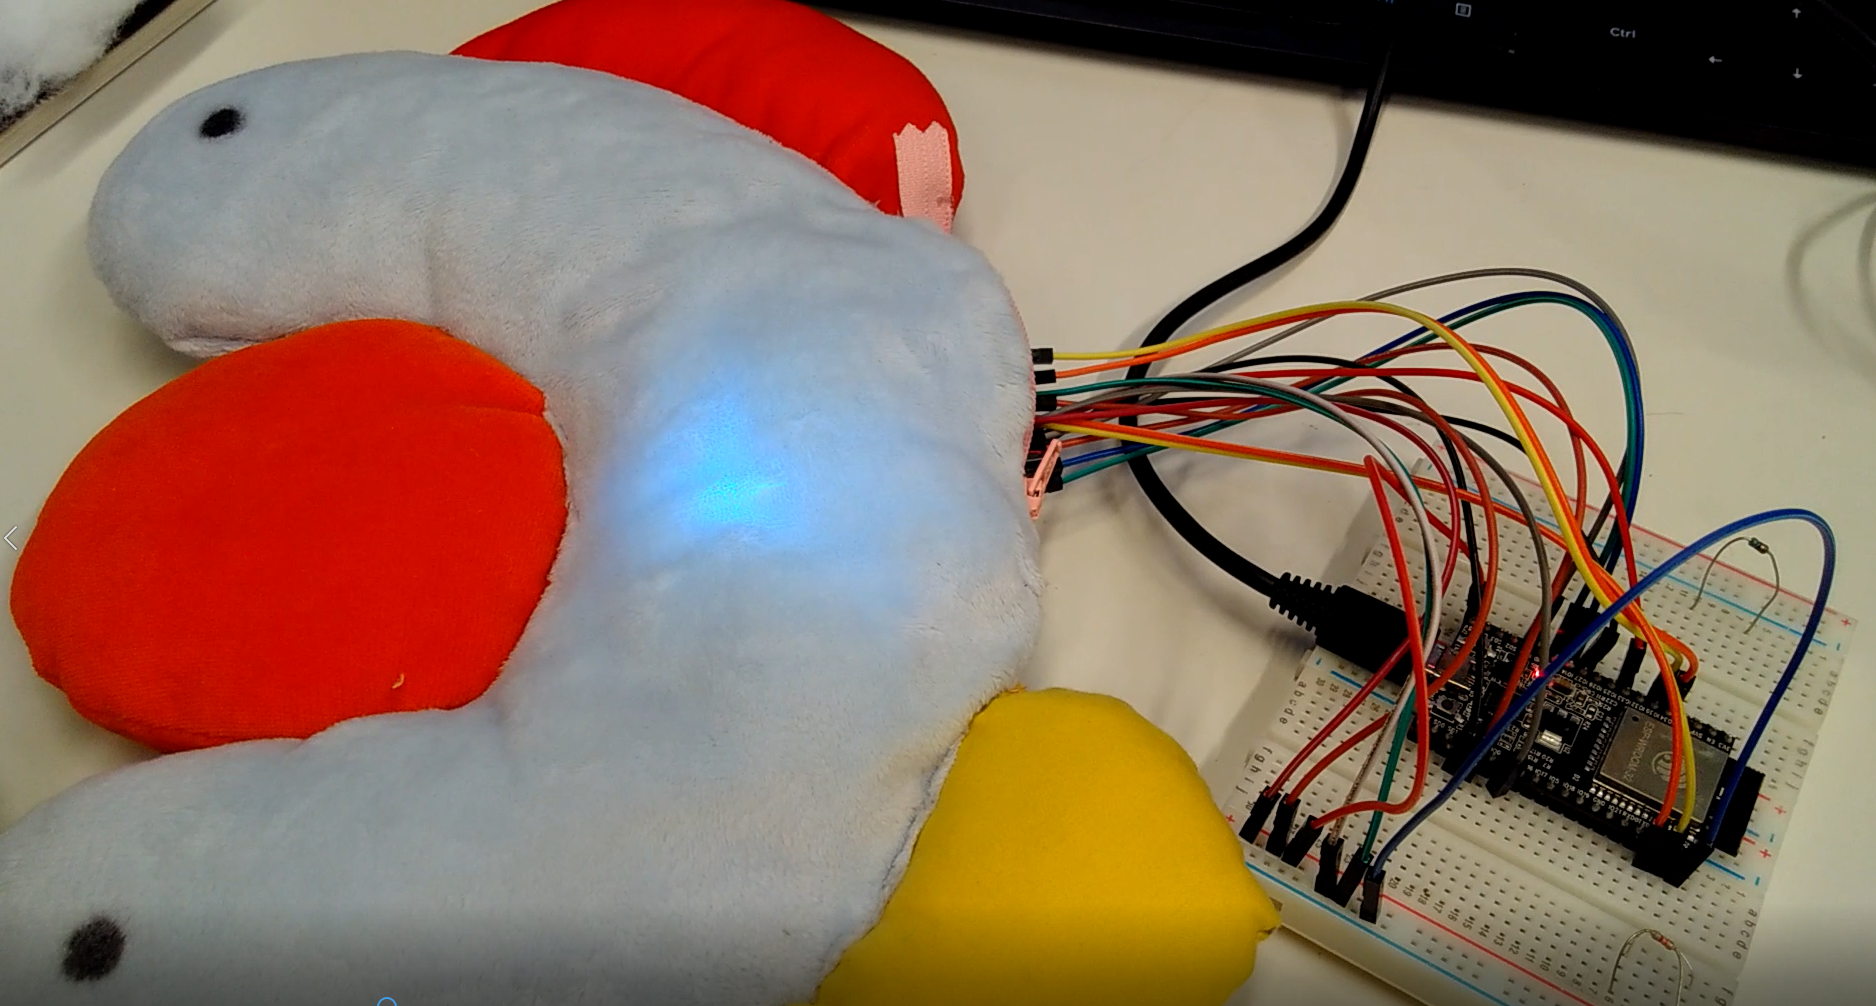
\includegraphics[width=0.8\textwidth]{images/HW/proto2_soft.PNG}
    \caption{Second prototype of our connected plush toy, as presented at MS5.}
    \label{fig:proto2_kid}
\end{figure}

\subsection{Prototyping iterations}

\subsubsection{First iteration: MS4}

Our first iteration of the soft PCB had stuffing between each layer of the soft PCB. The capacitive touch sensors were made out of sewn conductive fabric connected with conductive thread to connection pads. These pads were connected to the microcontroller board through safety pin connectors as pictured in Fig. \ref{fig:proto1}. As we only had SMD LEDs, we added sewable legs to connect them to the soft PCB, but they were too rigid and broke easily resulting in only one LED working on the first prototype.


\begin{figure}[ht]
    \centering
    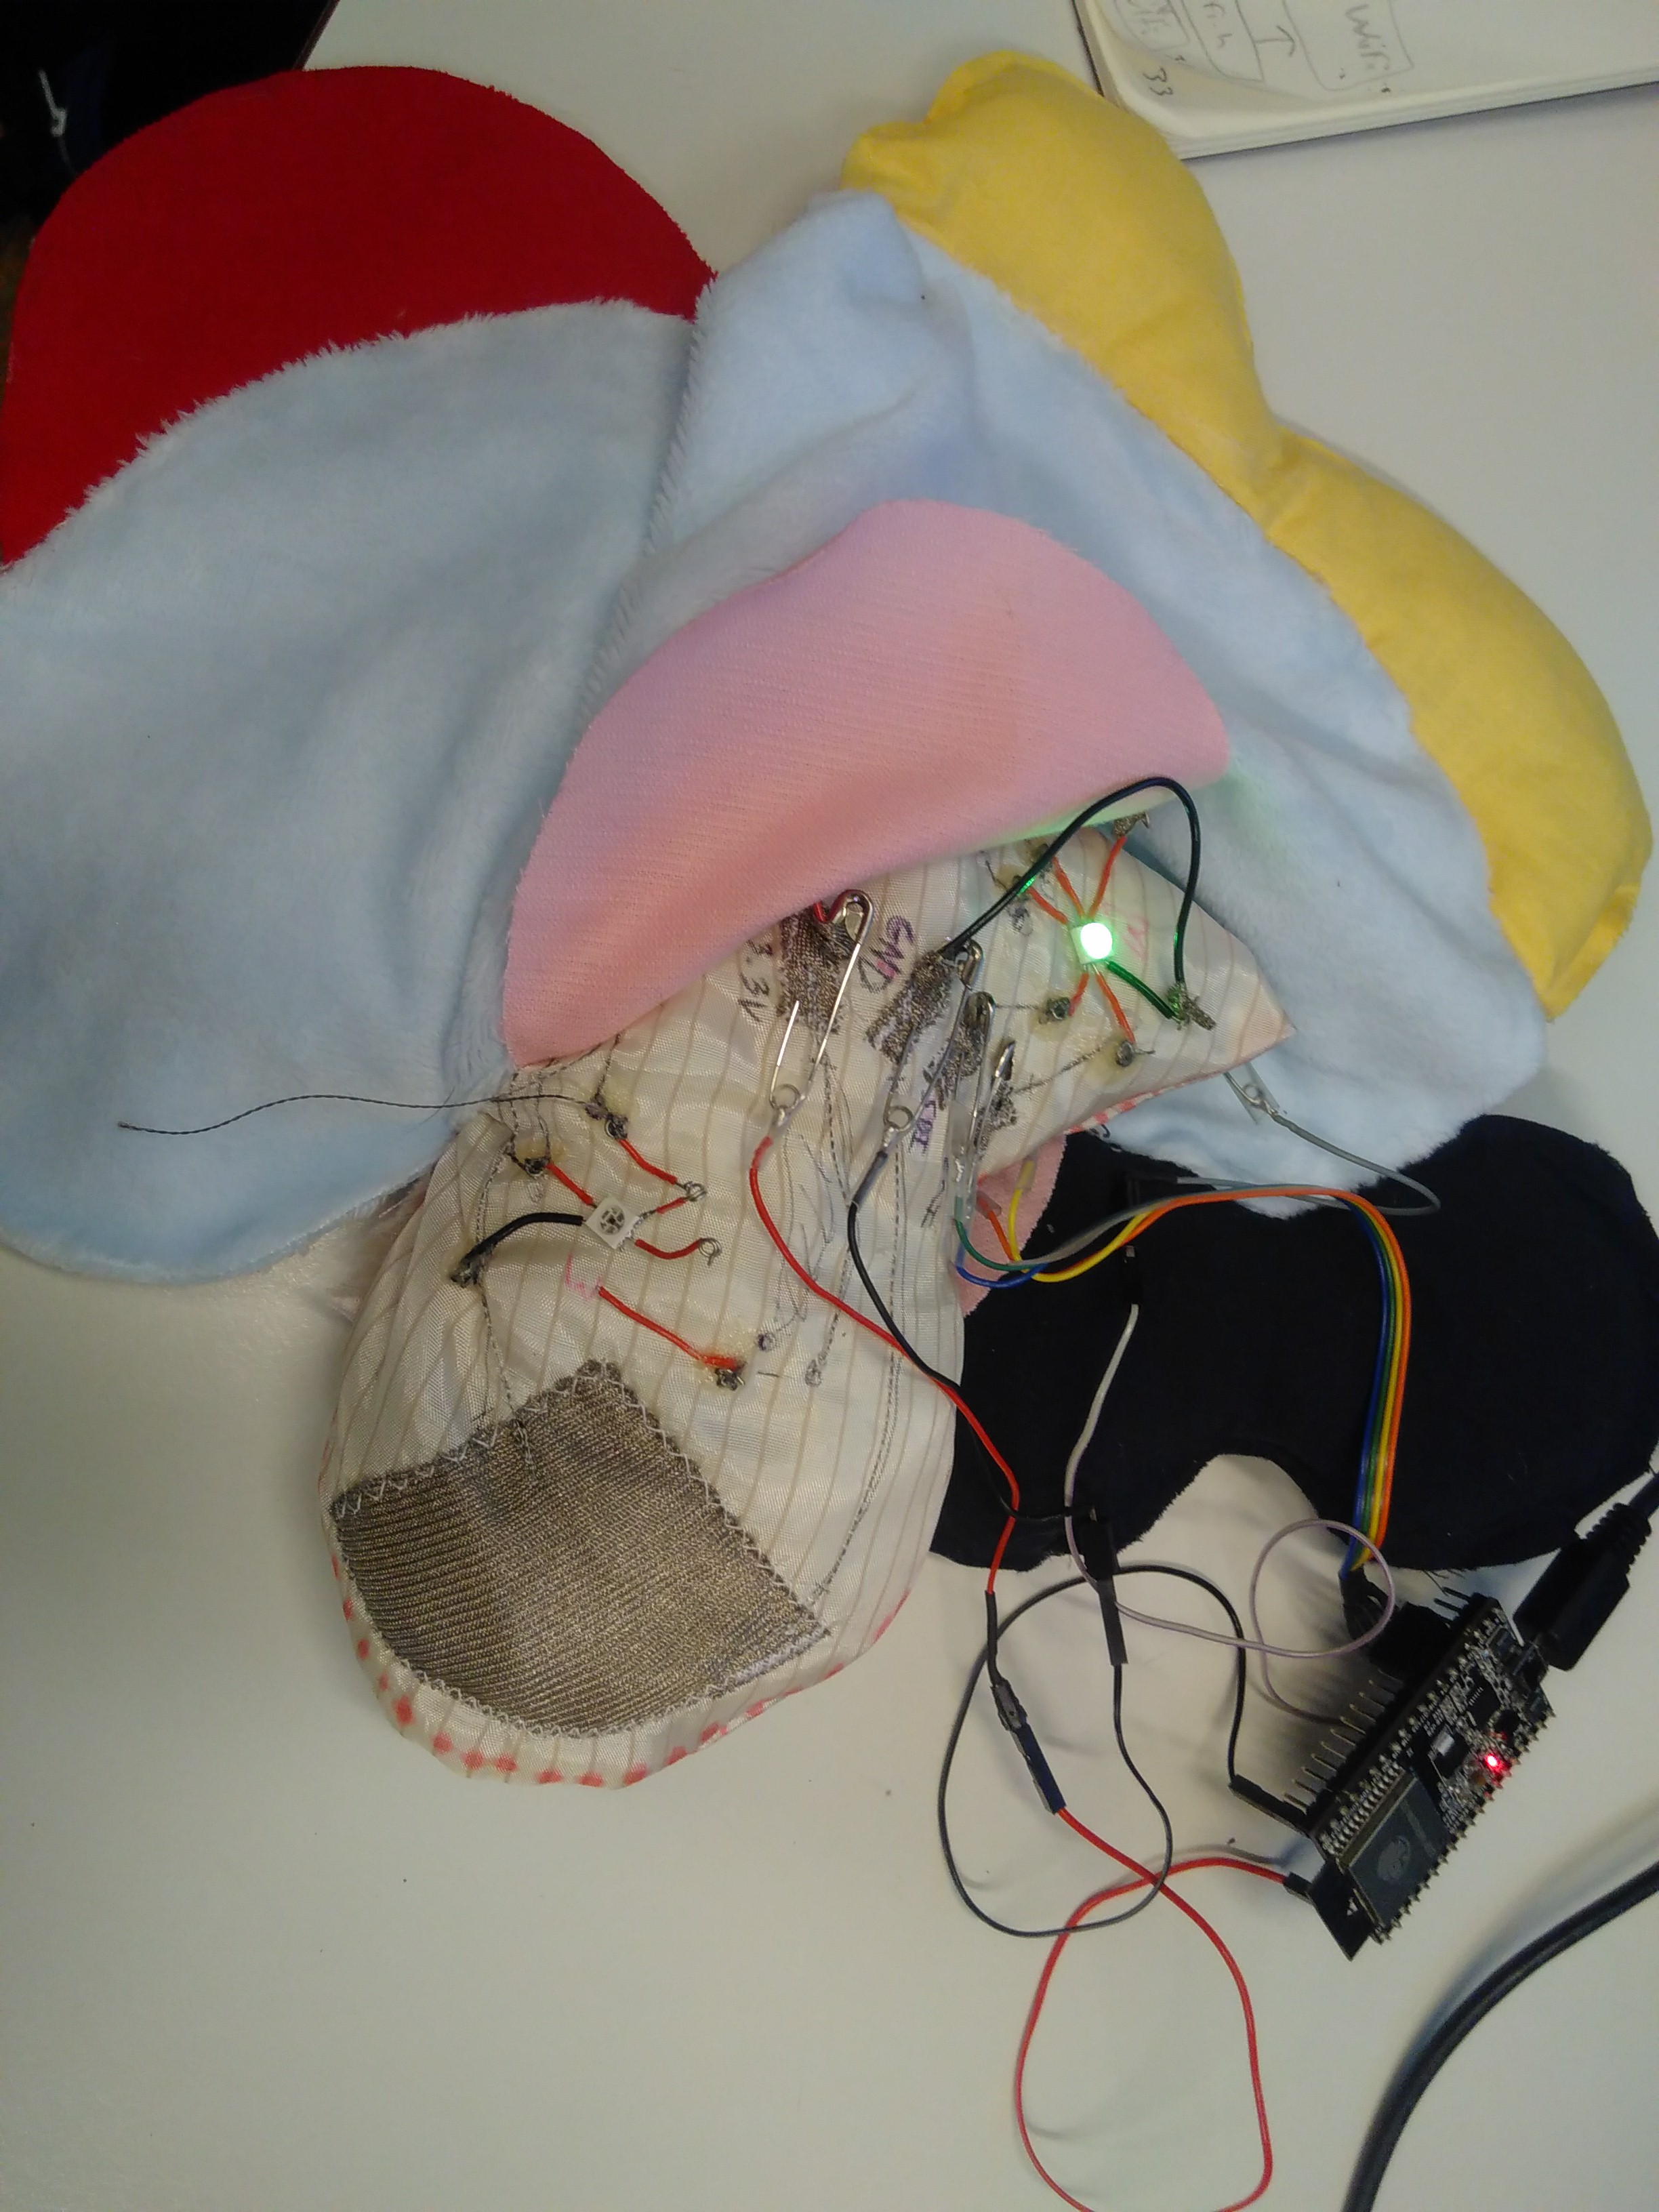
\includegraphics[width=0.4\textwidth, angle=90]{images/HW/proto1_connectors.jpg}
    \caption{First iteration of the soft PCB for MS4}
    \label{fig:proto1}
\end{figure}



\subsubsection{Second iteration: MS5}

For our second iteration of the soft PCB prototype, we decided to keep the soft PCB in two flat layers, one for sensors and one for LEDs, with an insulating layer in between. The touch sensors were made out of heat-bond conductive fabric \cite{heatbond}. The LEDs and sensors were connected with conductive thread, which was tied to crimp pins in housing ensuring proper connectivity with the microcontroller board. 
For the demonstration, we made a separate prototype with touch sensors painting on textile and two LED strips, as seen in Figure \ref{fig:proto2_fun}. This prototype was fully functional and reactive for proper interactions.
\paragraph{Issues}The conductive thread was very painful and long to sew to the soft PCB, as every connection (nearly a hundred ones) had to be tied with a knot. Moreover, the thread frayed at its extremities creating short-circuits, thus only half of the LEDs worked. The close proximity of the touch sensors and connecting threads sometimes caused interference between sensors.
\paragraph{Possible solutions} For our next prototype, we will experiment with heat-bond tracks as shown in Fig. \ref{fig:heat_tracks} or solderable conductive thread. These would be less susceptible to fraying and be more easily manufacturable as they do not require tying knots for each connection and can be machine sewn for the conducive thread. We will also experiment with ground planes or ground threads around the conductive touch sensors to limit interferences. 


\begin{figure}[ht]
    \centering
    \subfloat[Soft PCB on second prototype: LEDs layer\label{fig:proto2_LEDs}]{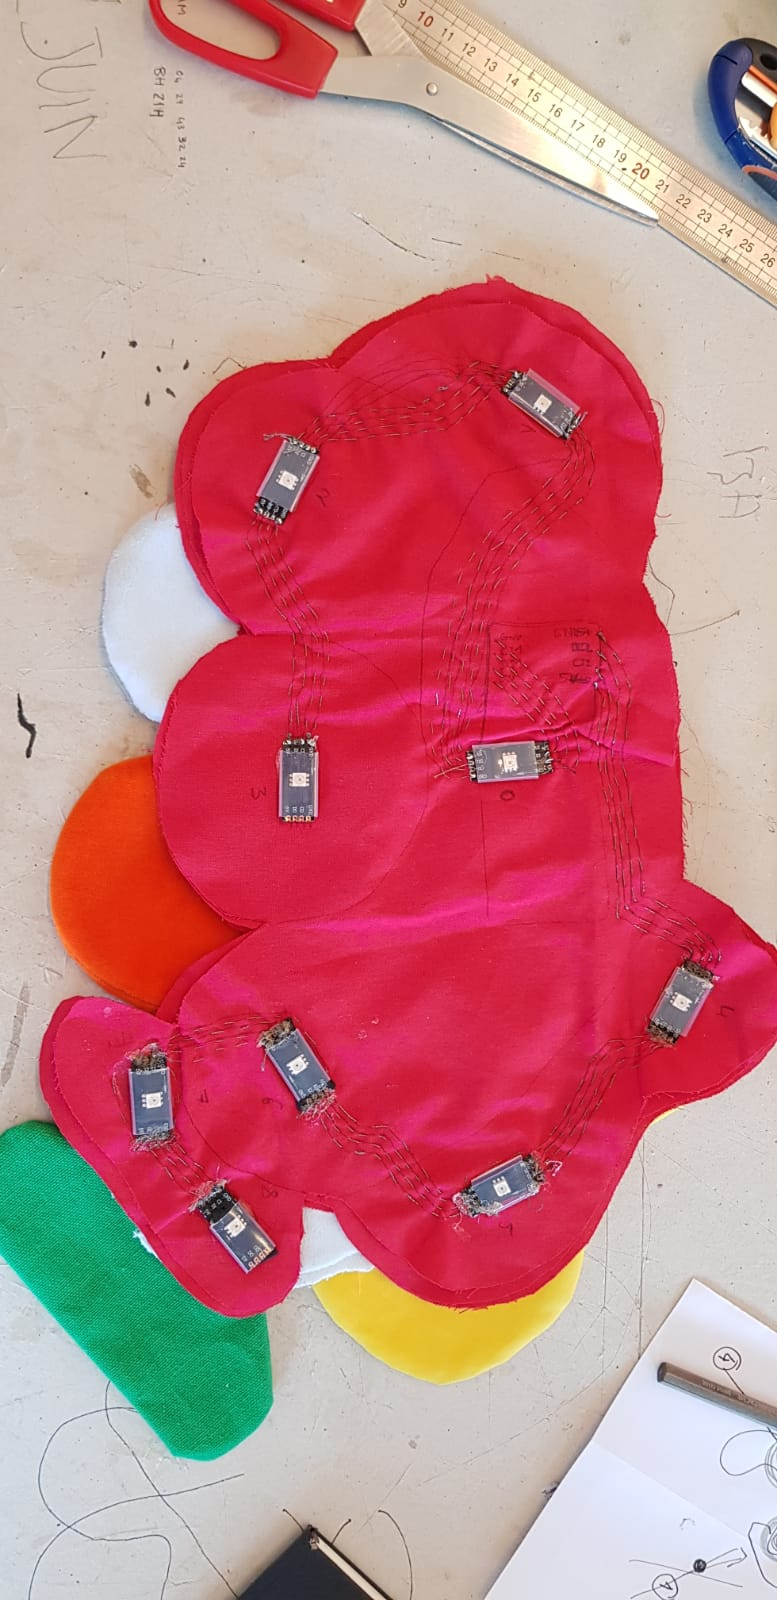
\includegraphics[width=0.27\textwidth, angle=90]{images/HW/softPCB_LEDs2.jpg}}\hfill
    \subfloat[Soft PCB on second prototype: sensors layer\label{fig:proto2_sensors}]{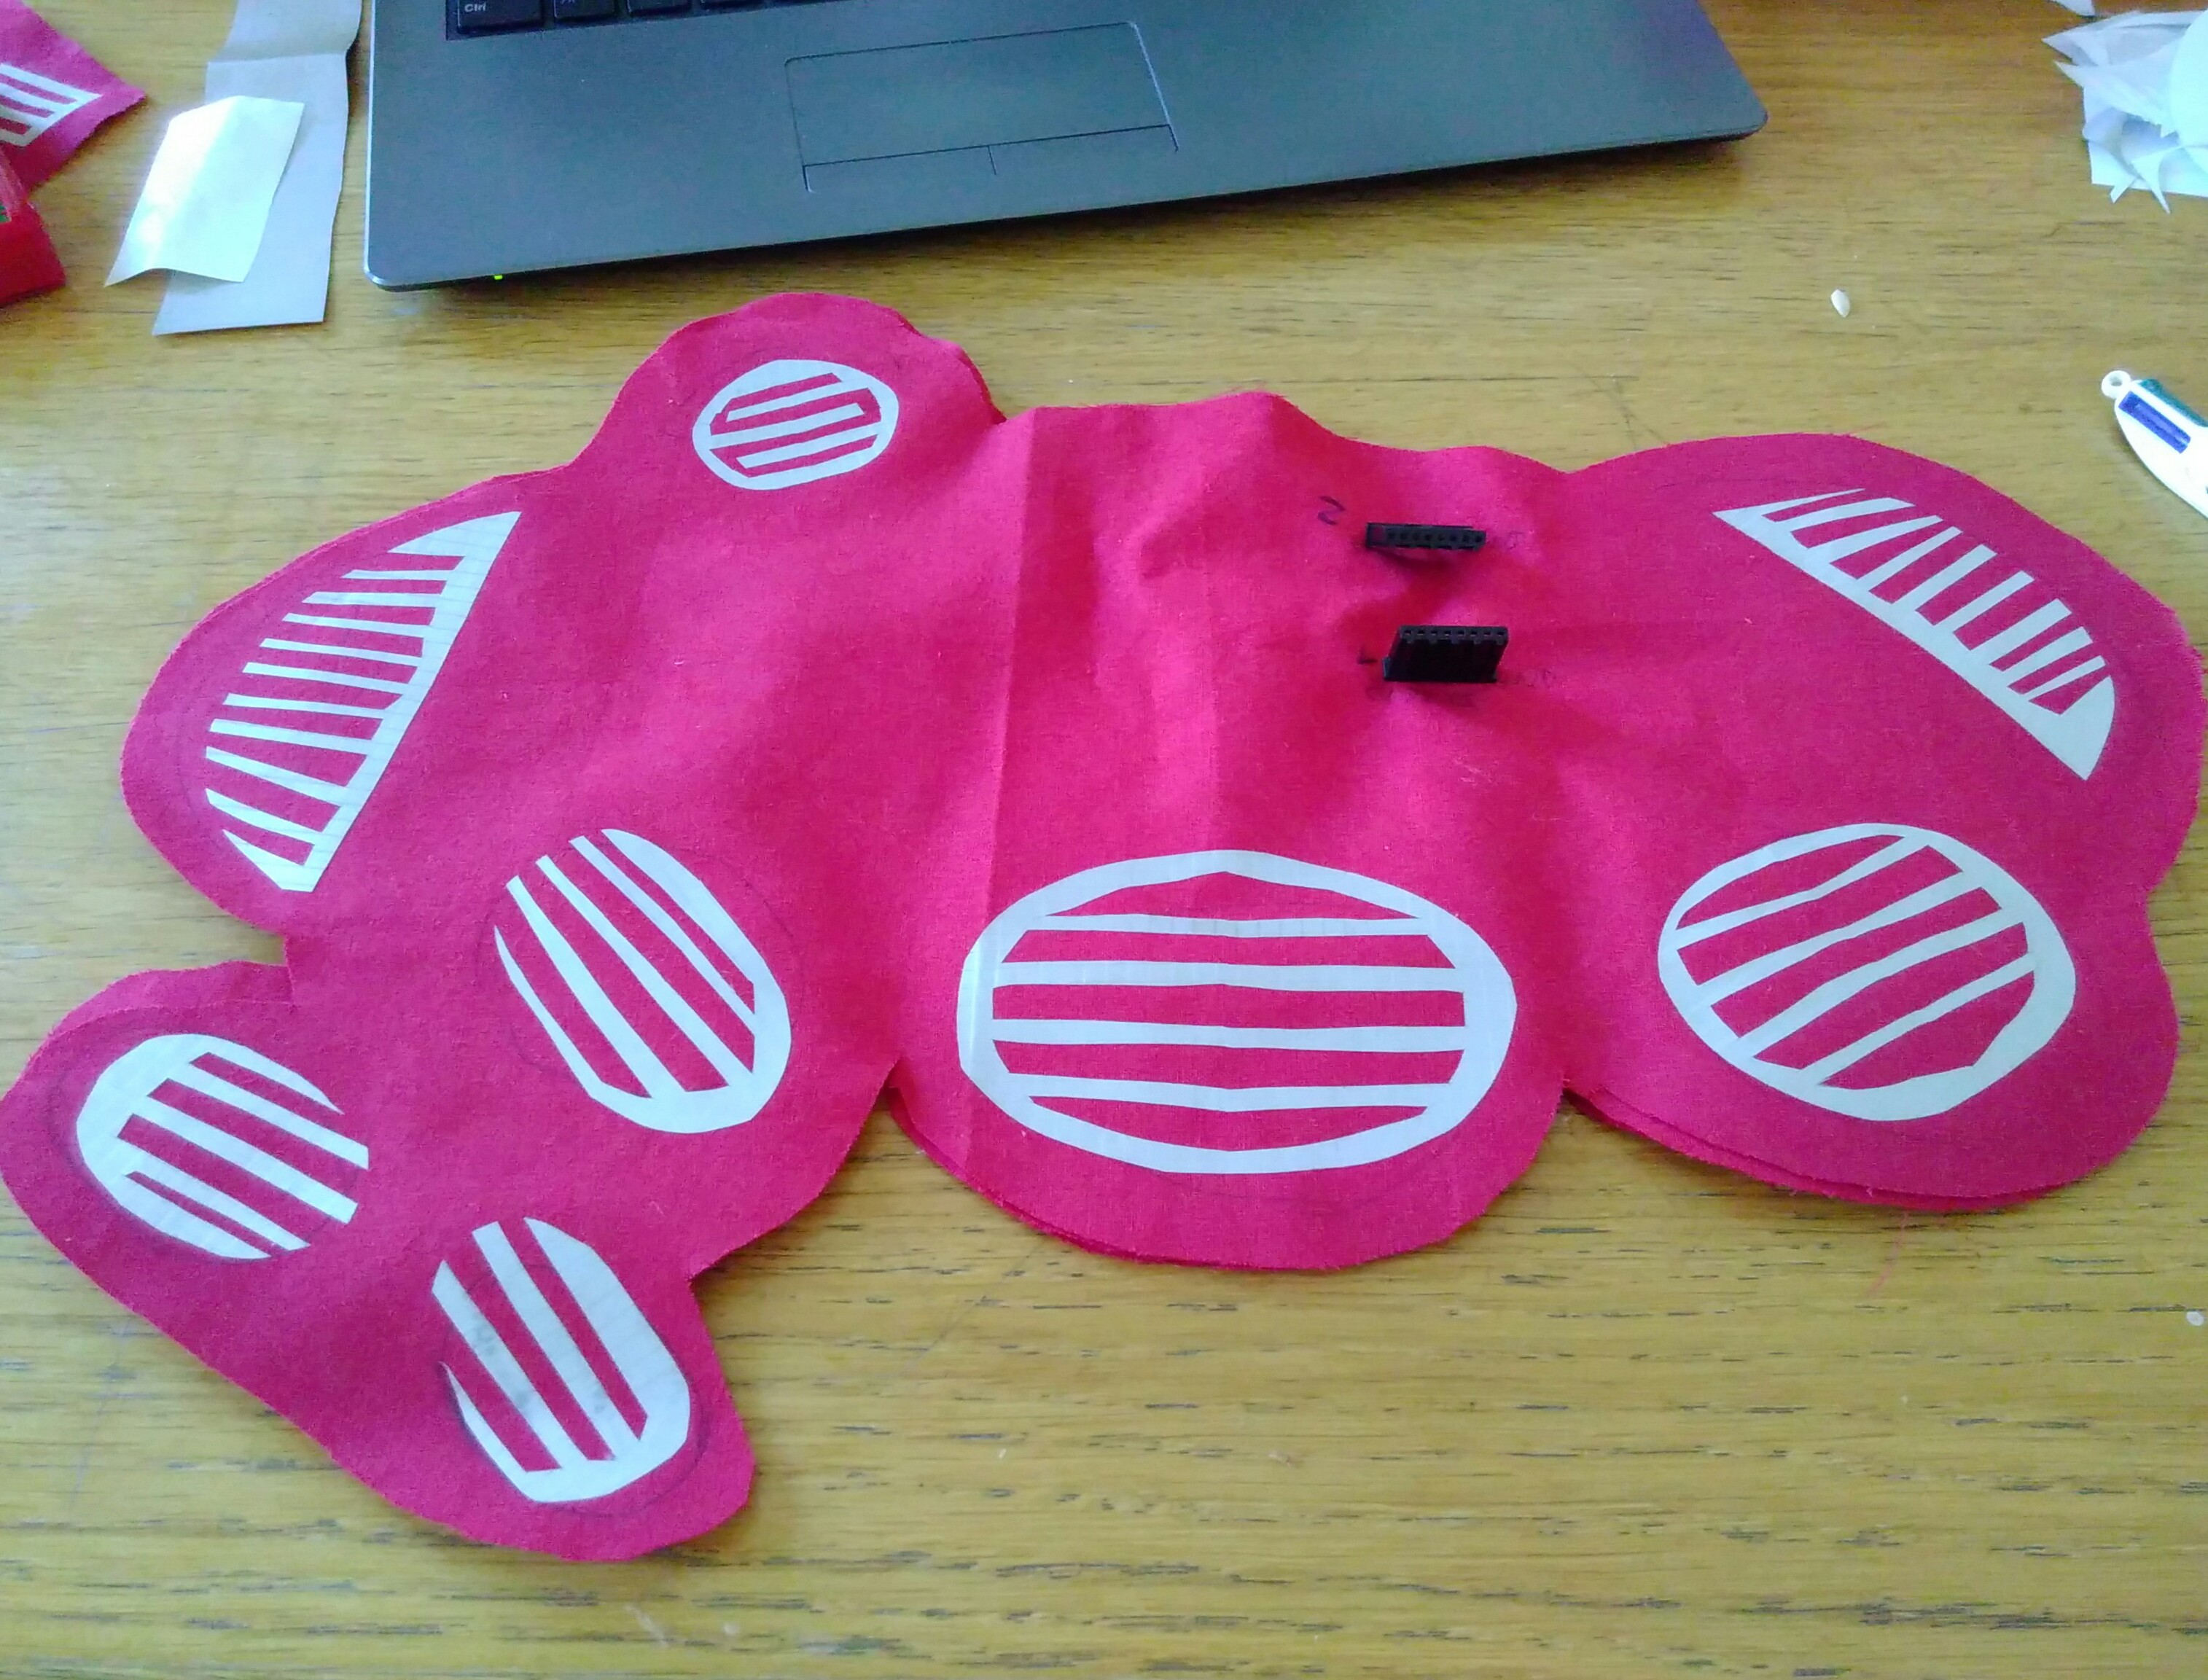
\includegraphics[width=0.4\textwidth, angle=0]{images/HW/softPCB_sensors2.jpg}}\hfill
    \subfloat[Crimp pins in housing\label{fig:proto2_connectors}]{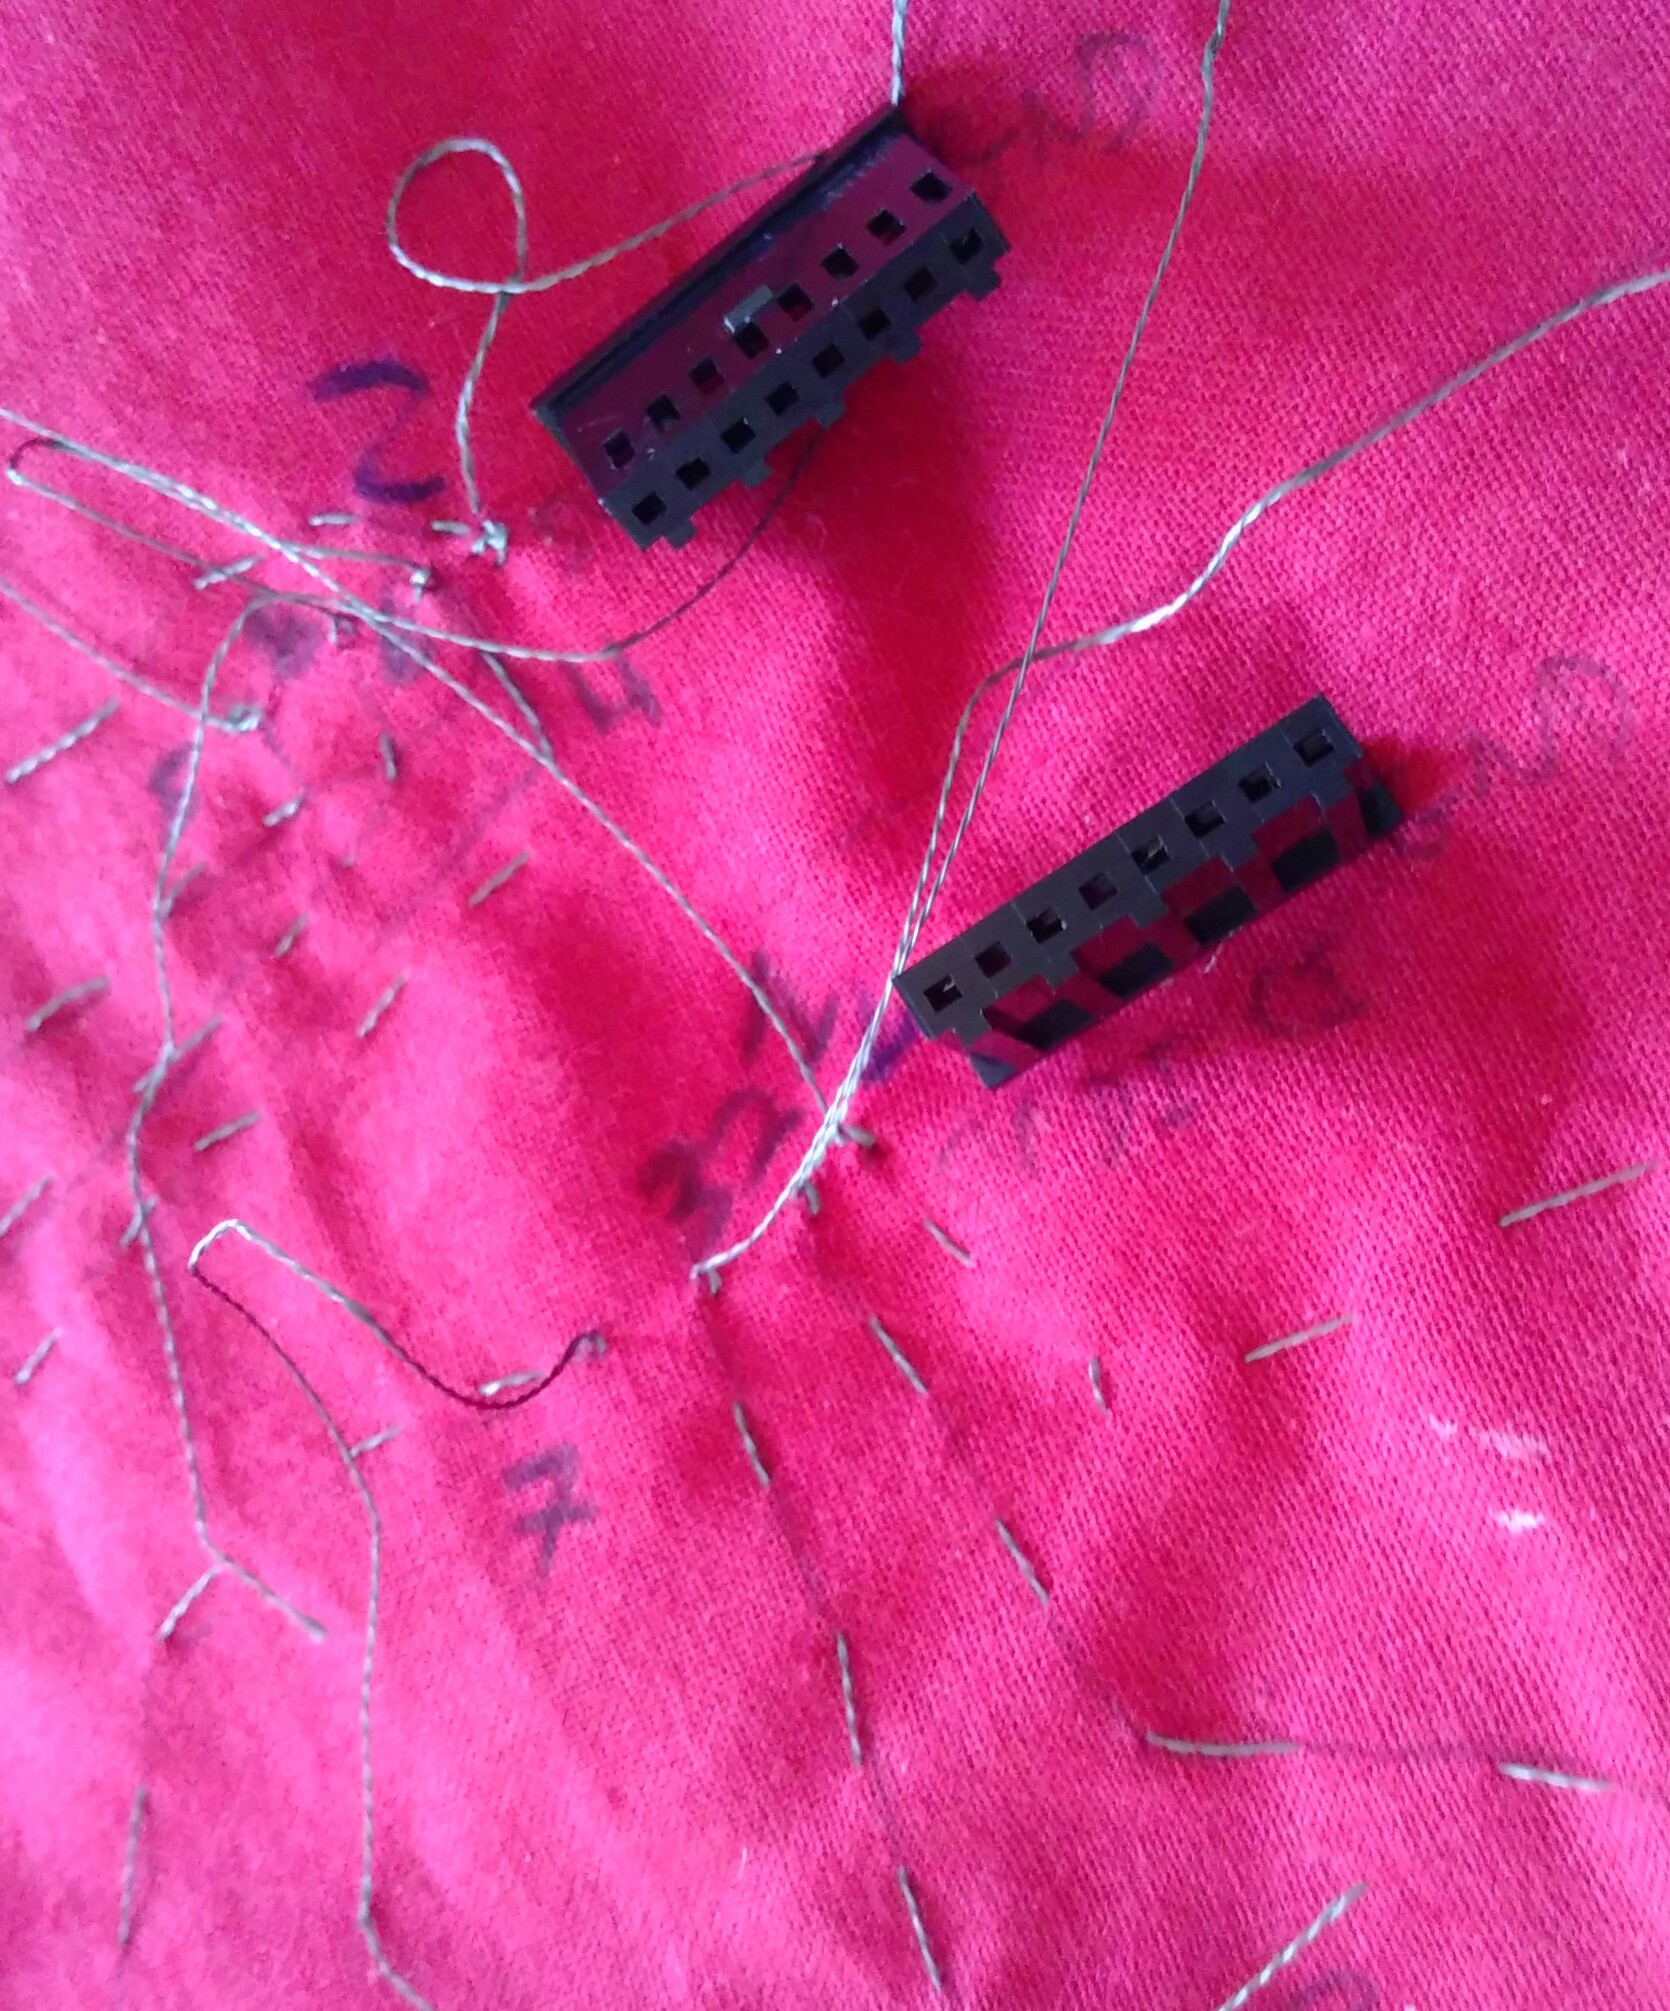
\includegraphics[width=0.3\textwidth, angle=90]{images/HW/proto2_connectors.jpg}}\hfill
    \subfloat[Interactive prototype\label{fig:proto2_fun}]{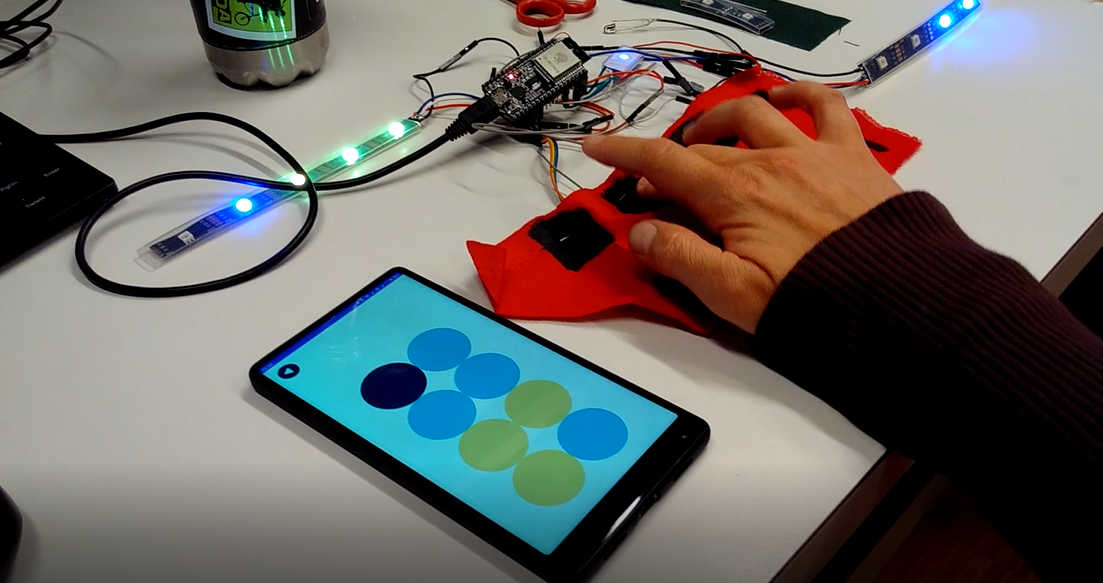
\includegraphics[width=0.55\textwidth]{images/HW/proto2_elec.PNG}}\hfill
    \caption{Second iteration of the soft PCB for MS5}
    \label{fig:proto2}
\end{figure}

\subsection{Blackbox design}
The 3D modelling of the blackbox was carried on by Marjane as part of her industrial design tasks. However, we collaborated closely on brainstorming, defining shapes, connectivity and positioning of the blackbox in the prototype. 

\begin{figure}[ht]
    \centering
    \subfloat[3D rendering\label{fig:blackbox_3D}]{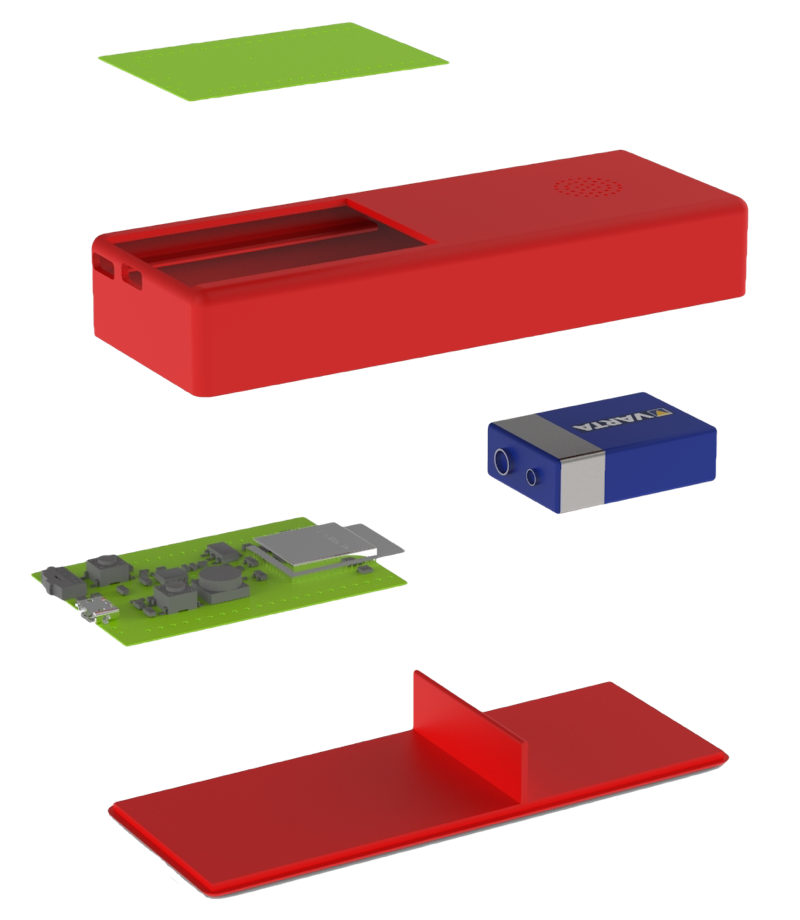
\includegraphics[width=0.35\textwidth]{images/HW/blackbox_v1.png}}\hfill
    \subfloat[3D printed blackbox with 3D printed PCB\label{fig:blackbox_v1}]{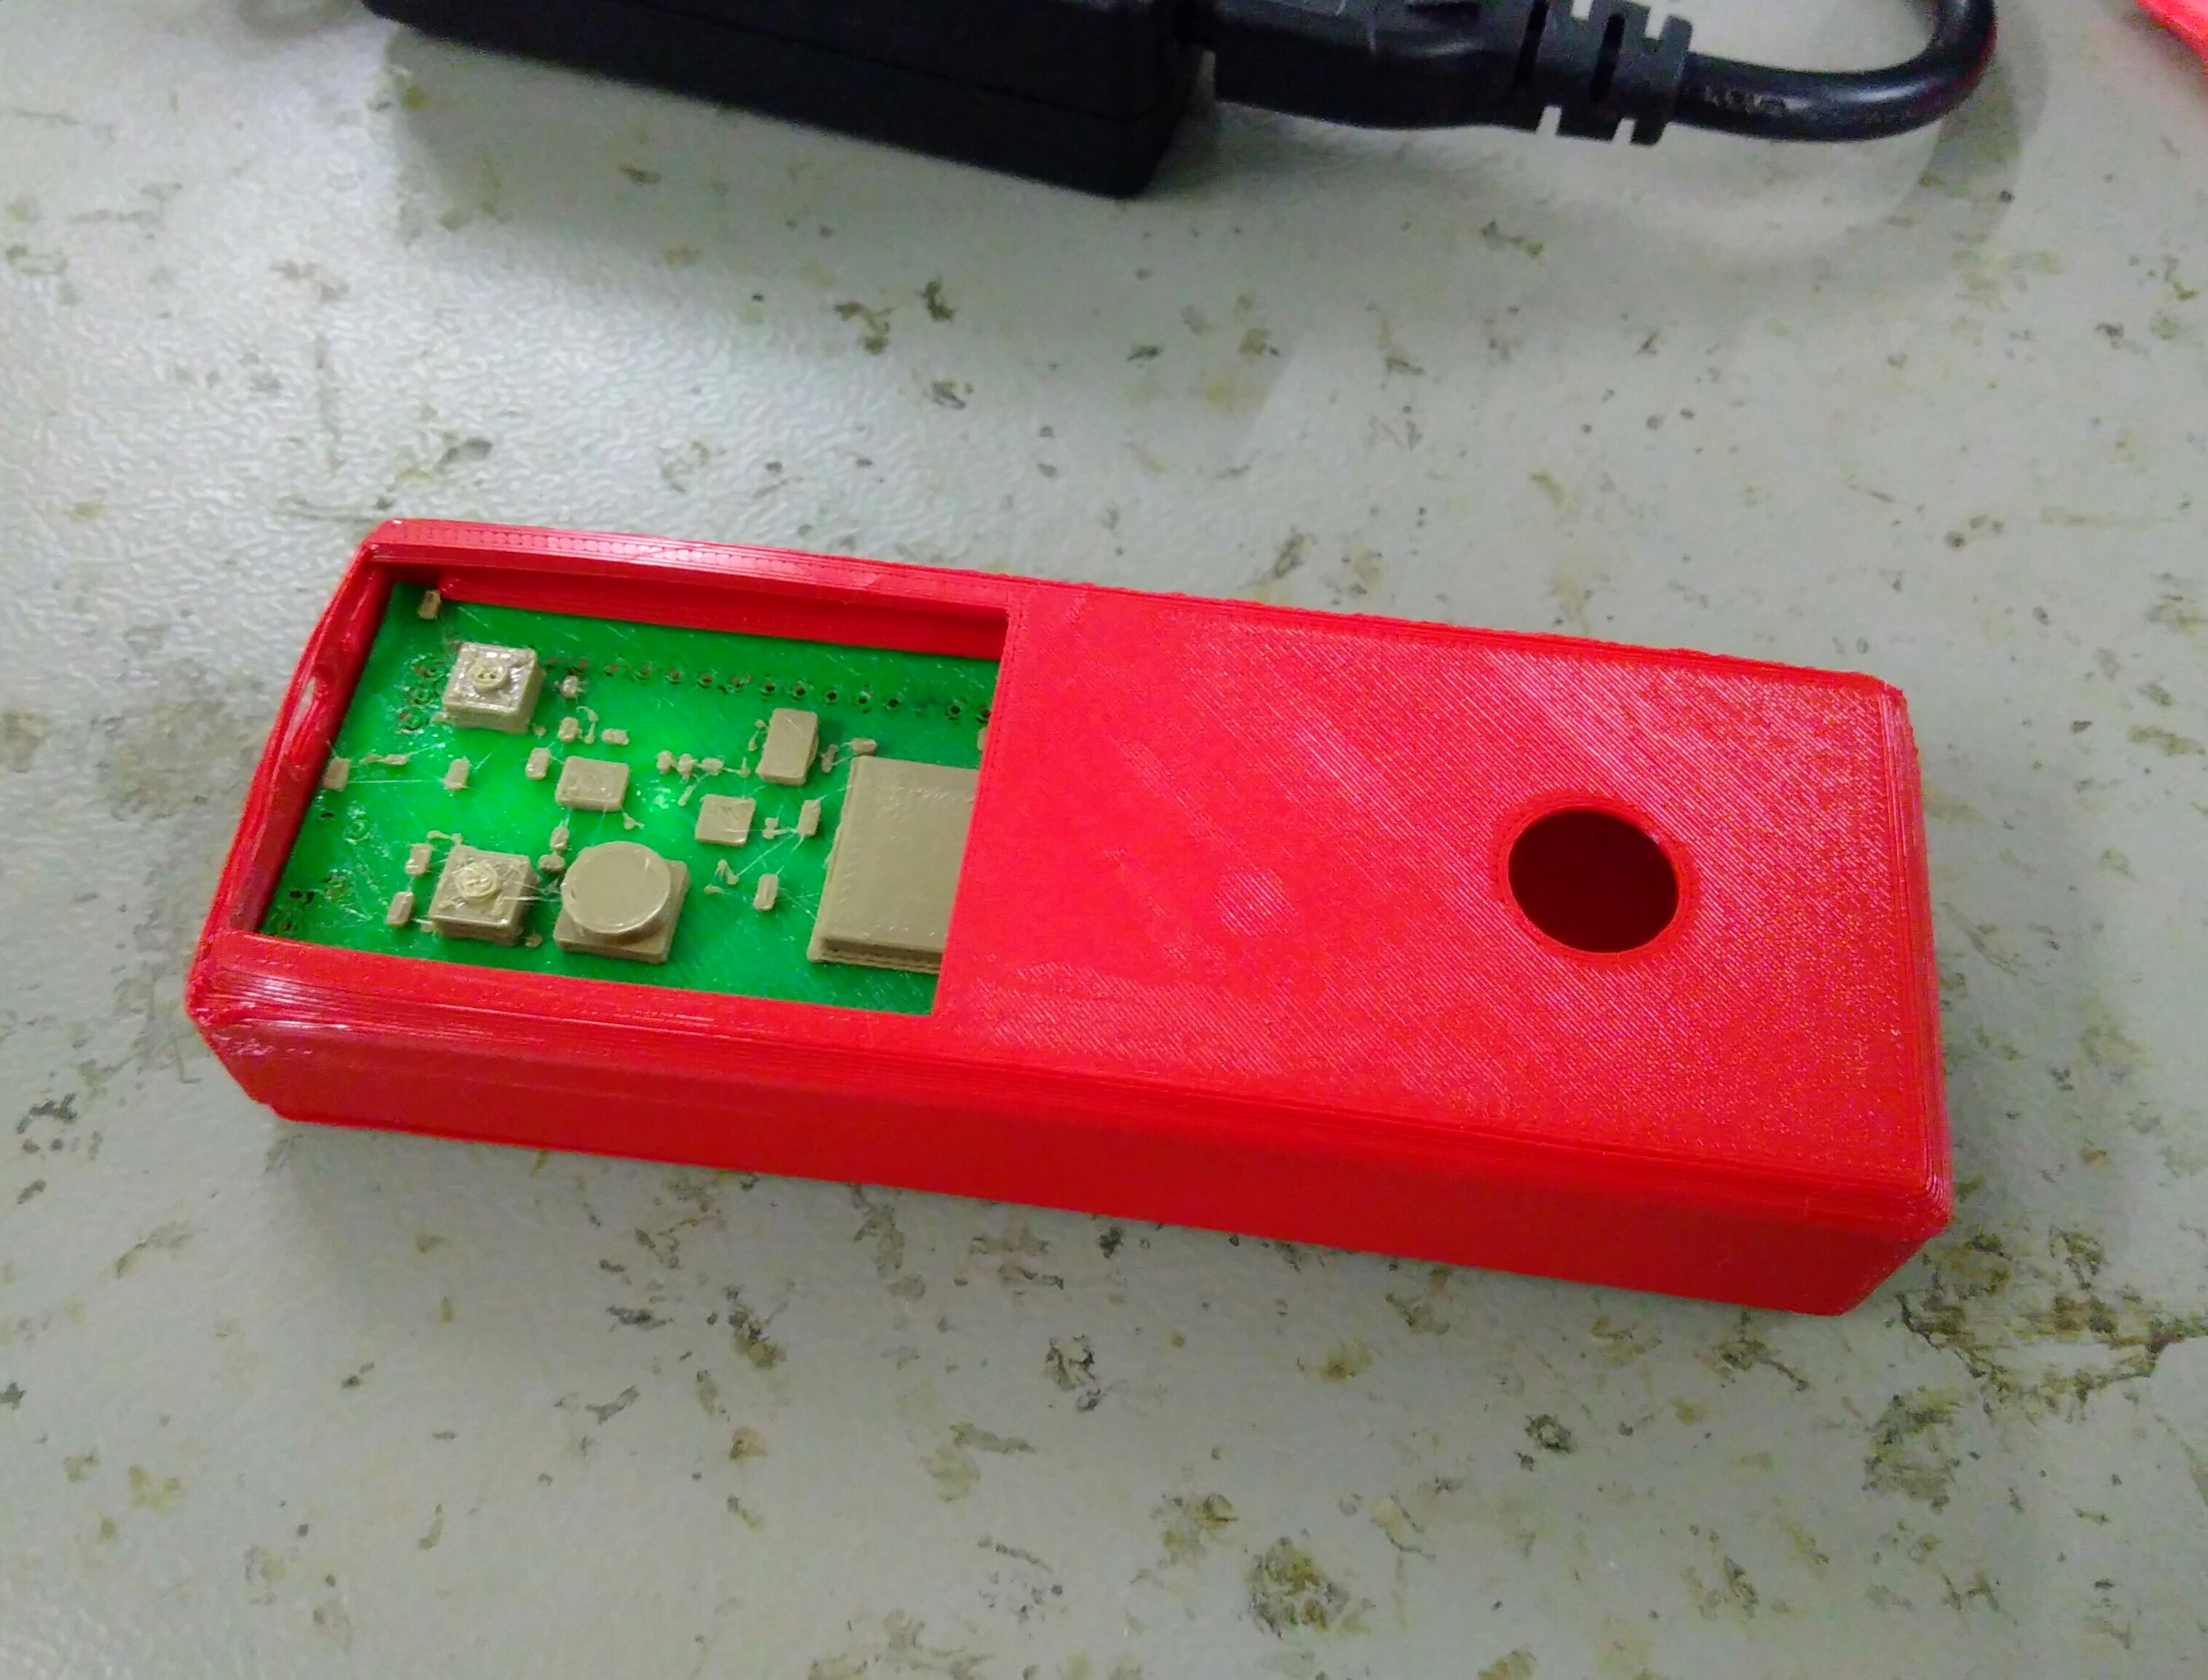
\includegraphics[width=0.6\textwidth]{images/HW/blackbox_3D.jpg}}\hfill
    \caption{First iteration of the blackbox design, including PCB, battery and loudspeaker}
    \label{fig:blackbox}
\end{figure}

\paragraph{Blackbox description} The blackbox holds the PCB, battery and speaker. It connects
to the Soft PCB through a secondary PCB breaking out the pin connections into textile conductors. The blackbox should be easily removable by the caretaker, giving easy access to the battery for replacement/recharging and be easy to connect to the the soft PCB. In our current version, the blackbox is connected to the soft pcb through pins; in a future version a more user-friendly connector will be considered.

\paragraph{Textile considerations}
The blackbox has to fit inside of a plush toy and be as little intrusive as possible. We decided to make the blackbox in a rounded, elongated ("banana") shape following the curves of the plush toy. A pocket accessible through a zipper is designed to hold the blackbox and define the connections with the soft PCB.

\begin{figure}[ht]
    \centering
    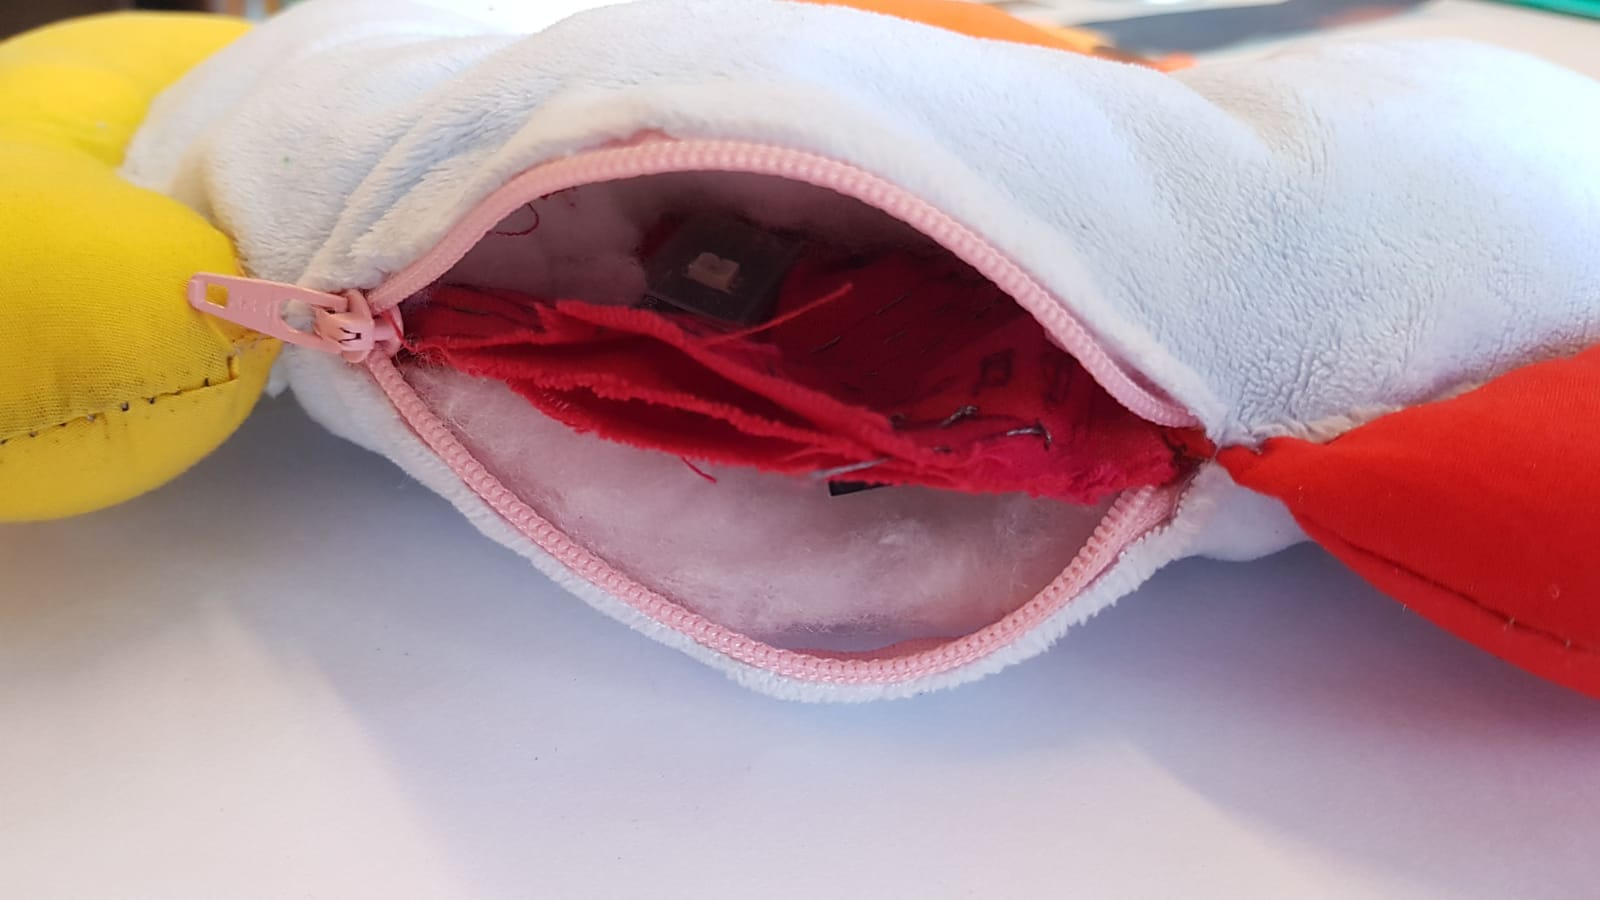
\includegraphics[width=0.6\textwidth]{images/HW/proto2_layers.jpg}
    \caption{Layers of the second prototype: outer skin, plush stuffing and soft PCB}
    \label{fig:p2_layers}
\end{figure}

    \paragraph{PCB design}
In our current version of the PCB (iteration 1), we decided to break out the circuit with many pins to keep prototyping options open for connectivity of hard to soft interfaces. The main PCB is linked to the Soft PCB through a secondary hard PCB, attached to the textile, to which conductive threads are tied, linking the elements (LED, sensors).
    
To achieve the smallest possible form factor, we decided to re-desing the shape of the PCB for a future version according to the desired shape of the blackbox. For this, we take into consideration the hard/soft connections, buttons, positioning of connectors, battery and speaker elements. 


\subsection{Soft PCB}\label{sec:softPCB} The "soft PCB" is a 3-layer, 2D fabric "PCB" with a first layer of textile and conductive touch pads, an insulating layer and a second textile layer with LEDs and conductive thread or textile conductor tracks linking the LEDs. The tracks are connected to pins in the current version of the prototype and will be linked to the secondary PCB in the next iteration of the prototype. In a future iteration of the prototype, we will consider a more compact, robust and user-friendly connector such as the one presented in Figure \ref{fig:fp_connector}.


\begin{figure}[H]
    \centering
    \subfloat[Textile capacitive sensors on soft PCB\label{fig:soft_capa}]{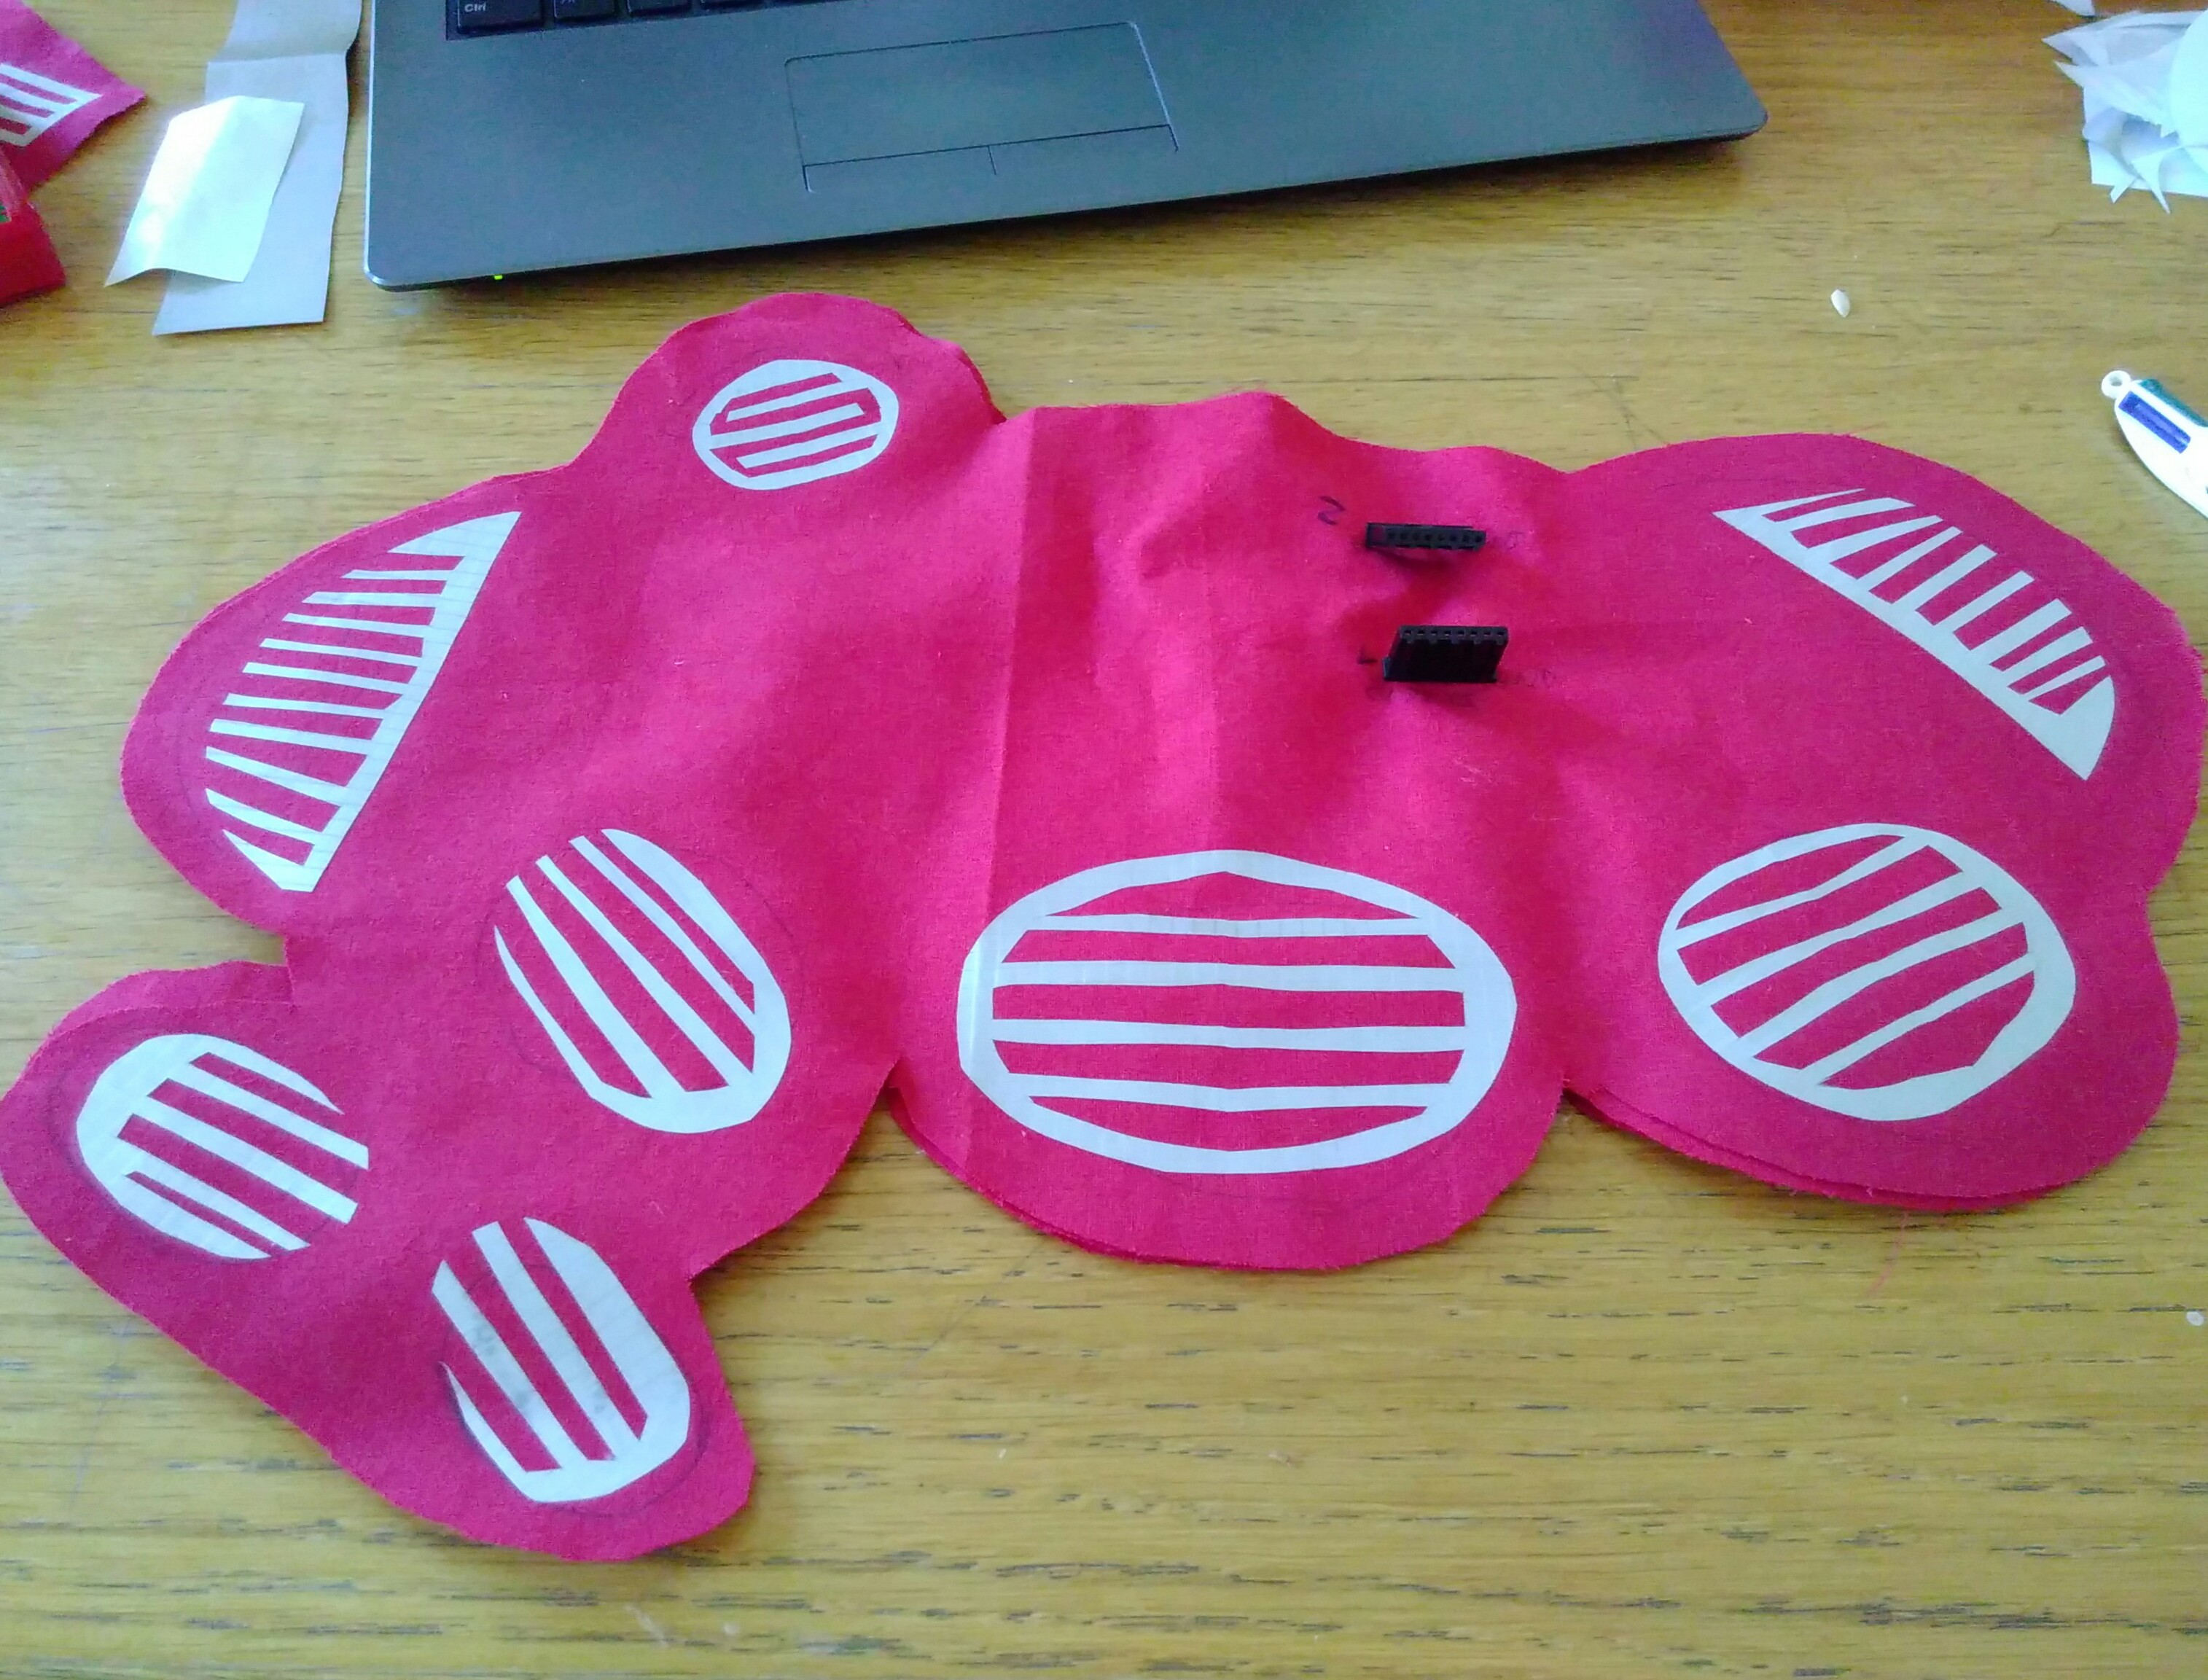
\includegraphics[width=0.47\textwidth]{images/HW/softPCB_sensors2.jpg}}\hfill
    \subfloat[Conductive thread linking the LEDs\label{fig:soft_threads}] {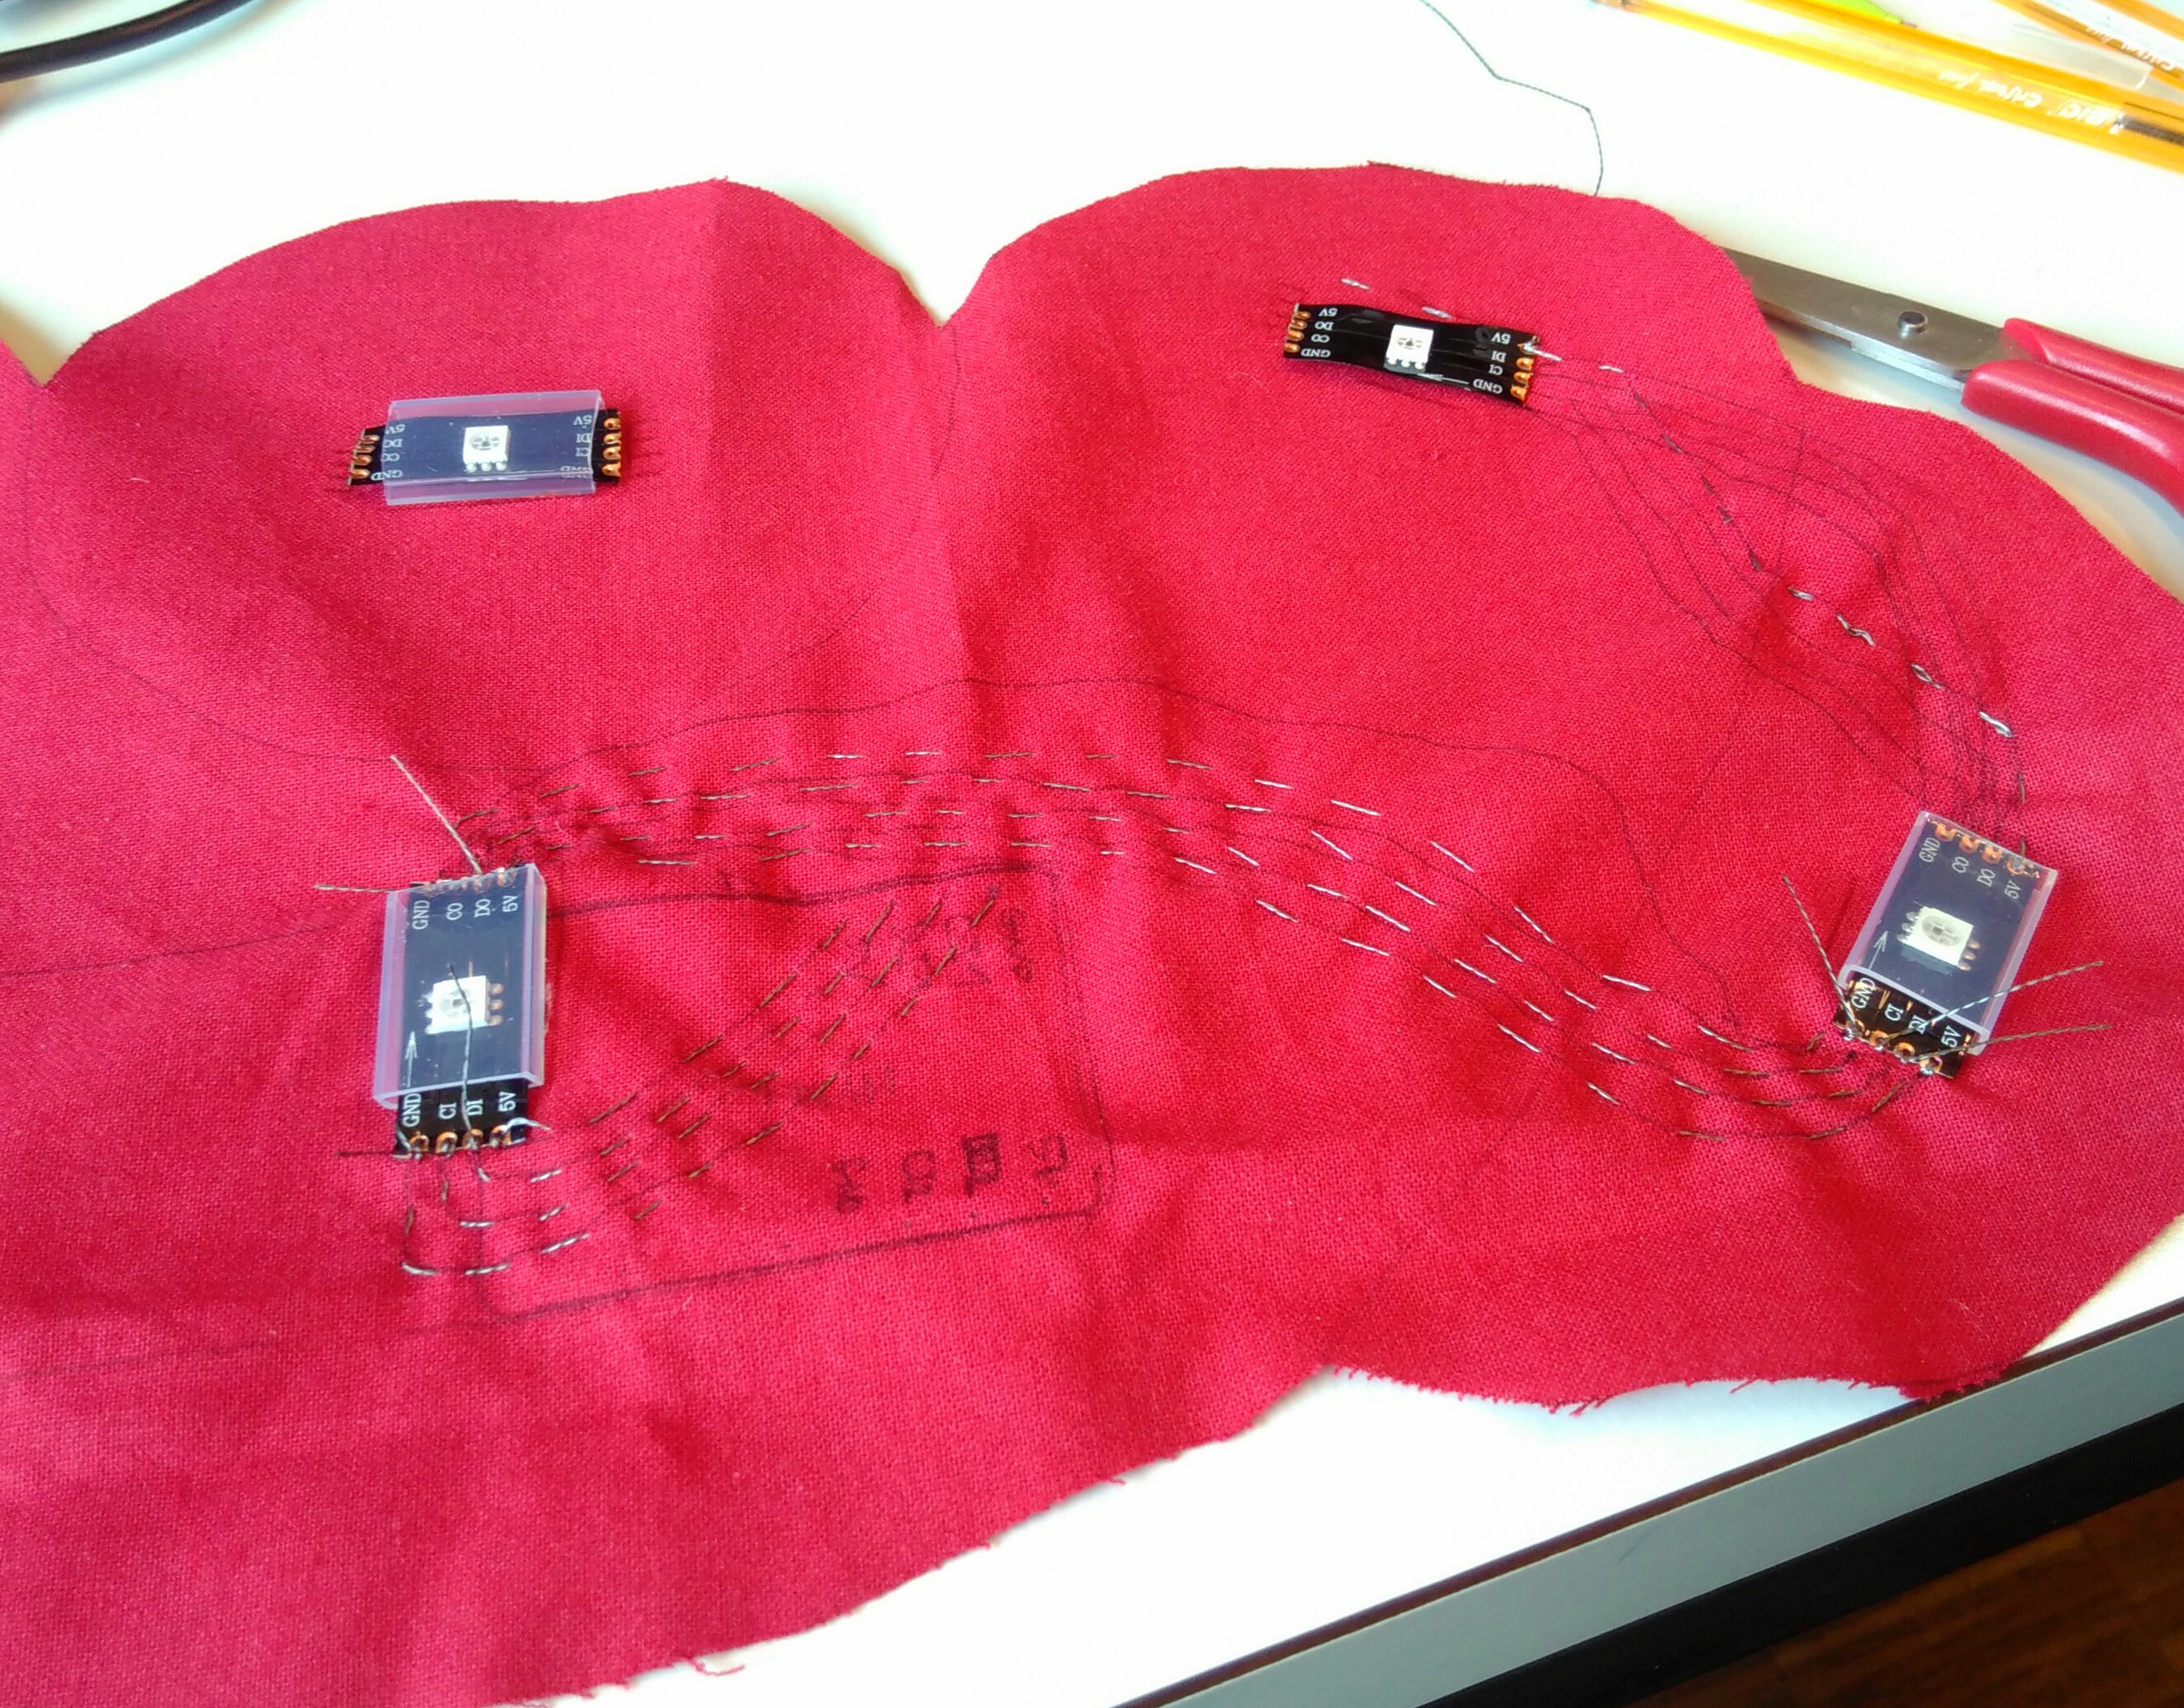
\includegraphics[width=0.47\textwidth]{images/HW/softPCB_LED_thread.jpg}}\hfill
    \caption{Details of top and lower layers of soft PCB} 
    \label{fig:soft_pcb}
\end{figure}

\subsubsection{Washability} Our goal for the plush toy is to be fully machine-washable once the blackbox is removed. The electronics (LEDs, connectors) would ideally be sealed in silicon while the textiles can endure a small number of washing cycles.

\subsubsection{Manufacturing options} For the first two prototypes, the LEDs were hand sewn to the soft PCB. The touch sensor pads were either machine sewn or heat-bonded to the textile support. As it is, the soft PCB takes several hours of tedious handwork to manufacture. We are currently experimenting with using the heat-bond conductive fabric on both sides of the soft PCB on which LEDs will be directly soldered (Fig. \ref{fig:heat_tracks}). Currently, this setup has been successfully tested with tracks slightly thinner than 1mm. However, the soldered connections prove to be very rigid compared to the textile support and may require strengthening.

\begin{figure}[ht]
    \centering
    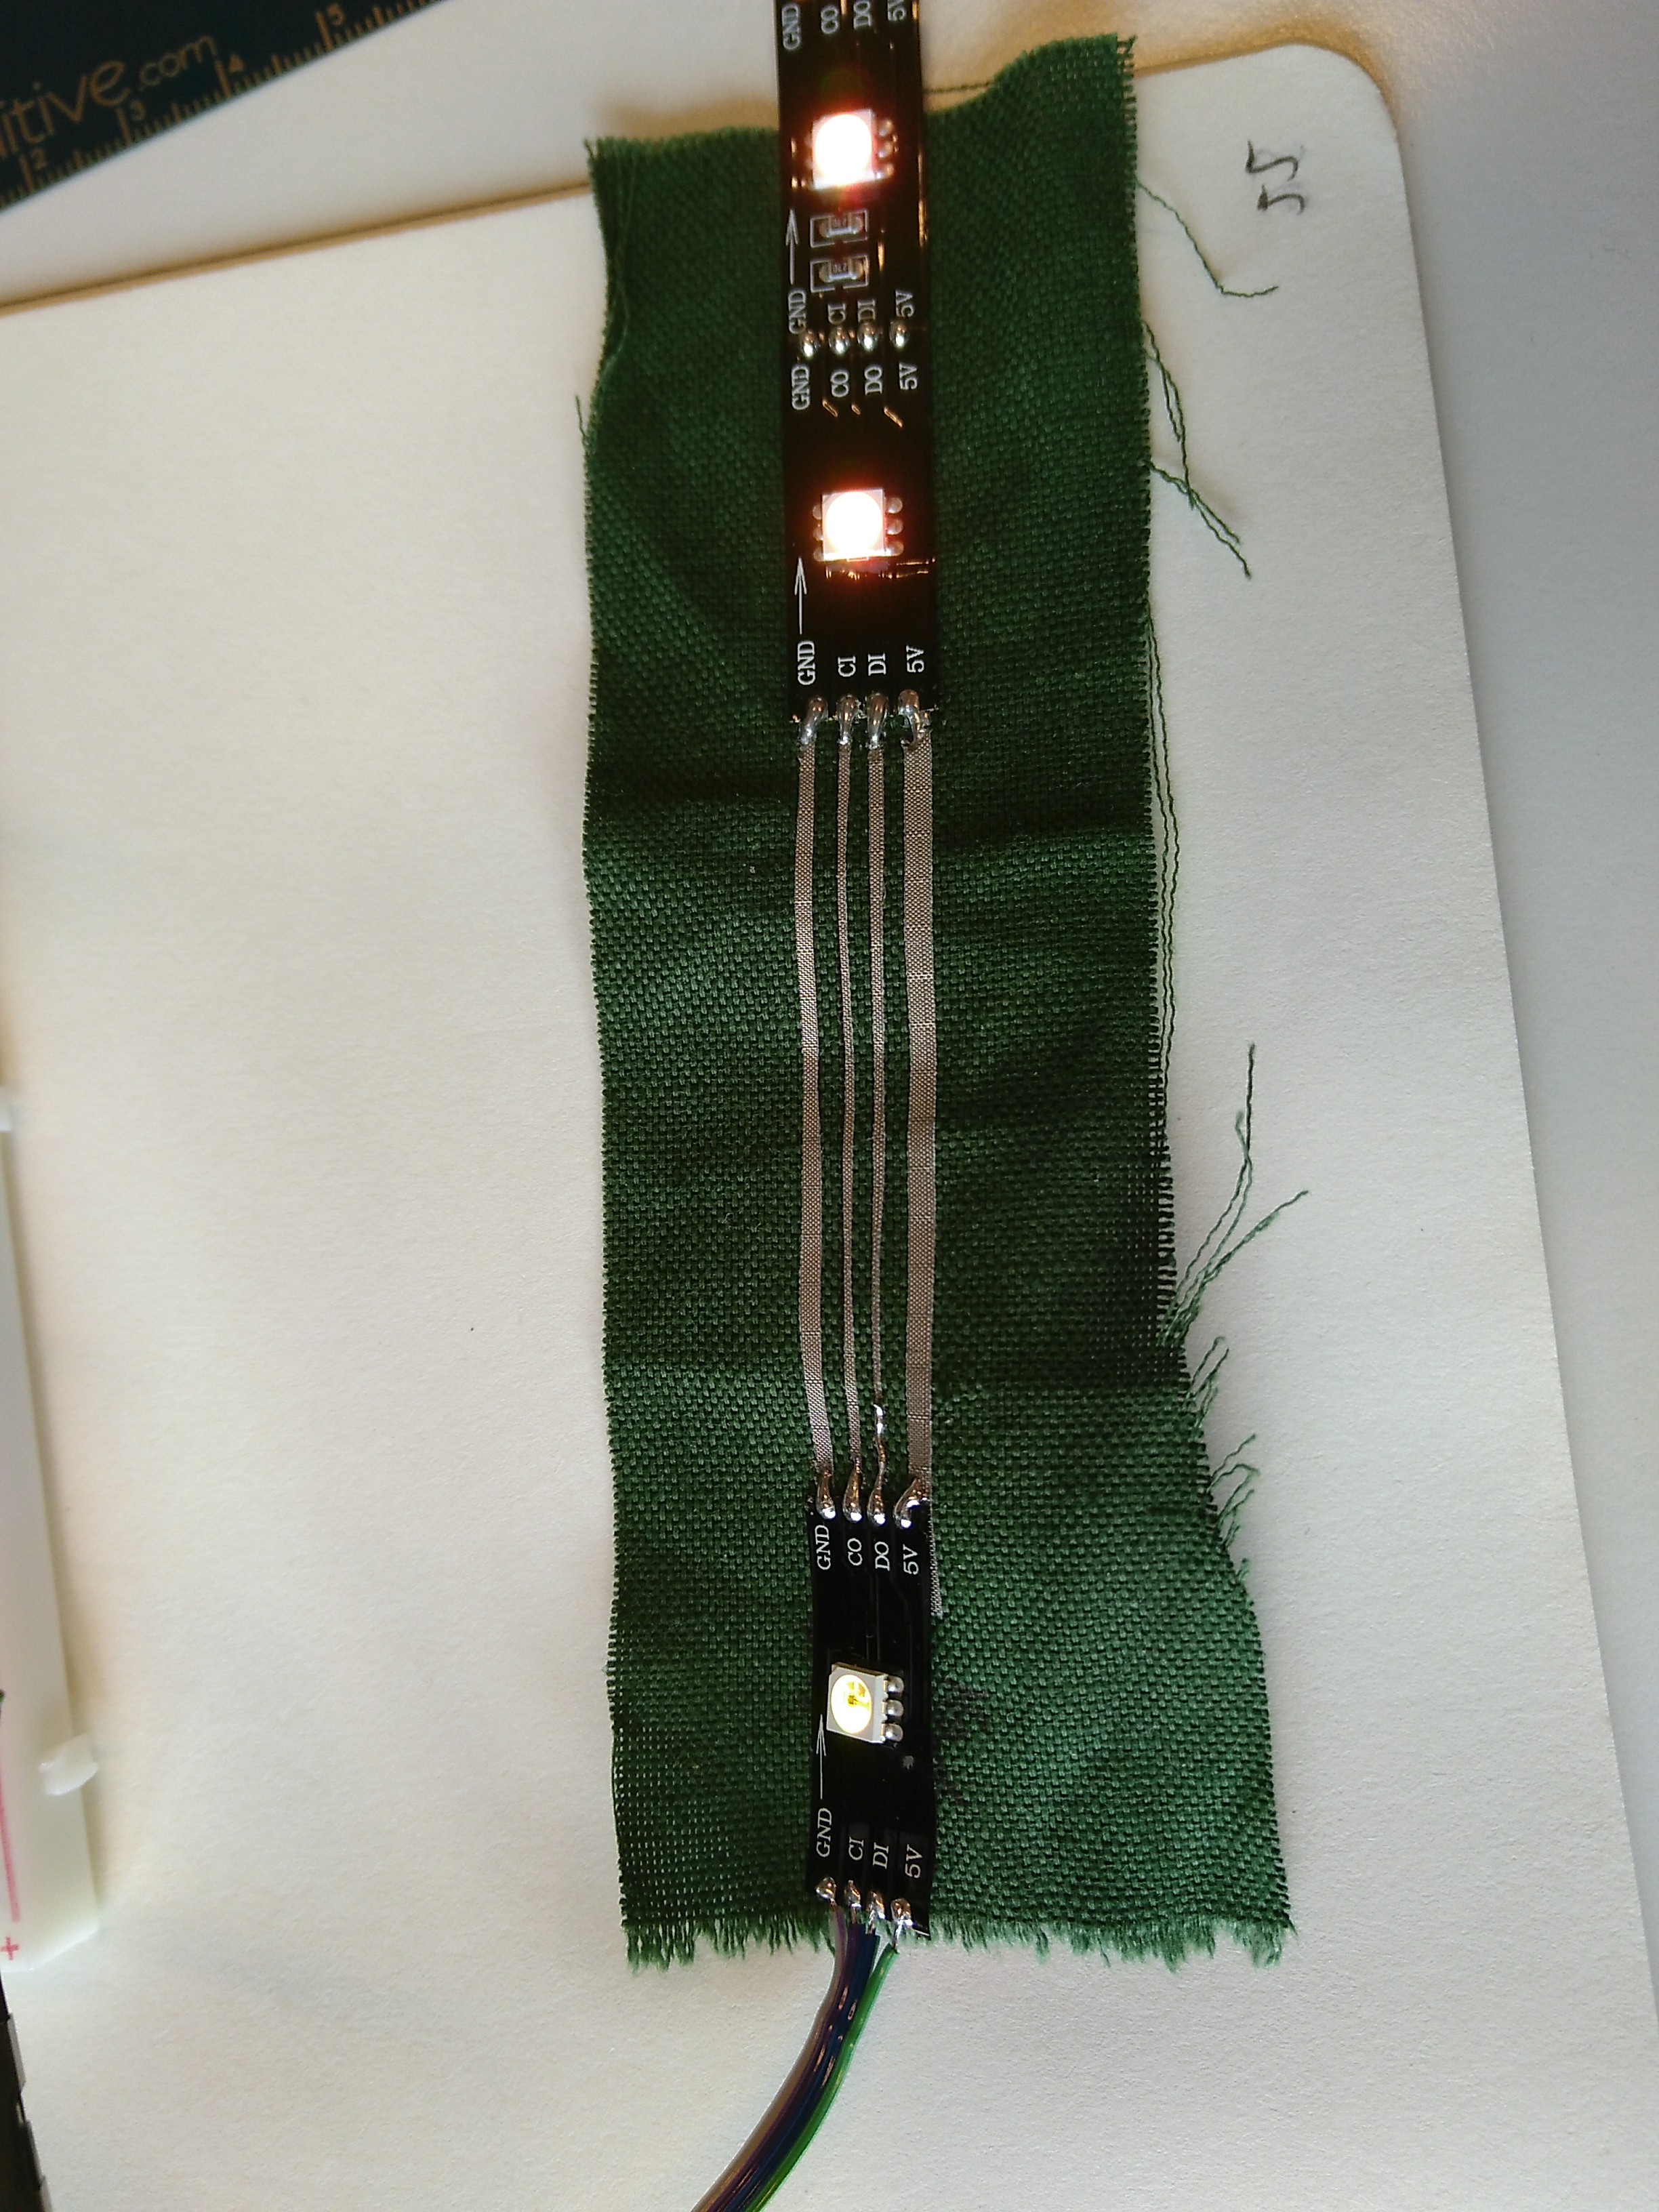
\includegraphics[width=0.6\textwidth, angle=-90]{images/HW/heatbond_tracks2.jpg}
    \caption{Test sample of heat-bonded conductive tracks}
    \label{fig:heat_tracks}
\end{figure}

\subsection{Soft sensors}
    \subsubsection{ESP32 integrated capacitive touch sensors}
In our project, we take advantage of the ESP32's built-in capacitive touch sensors. These are linked to conductive textile pads on the soft PCB. 
\medskip
Touch pad sensing on the ESP32 is handled by a hardware-implemented finite state machine (FSM). Touch pad sensing data can be obtained through checking registers in firmware or interruptions triggered by touch which can also wake up the CPU from deep sleep.

\paragraph{ESP32's capacitive touch sensors' working principle} 
The capacitance of each sensor is periodically charged then discharged. The swing slope is affected by touch, as a touched sensor has a high capacitance compared to an untouched one. At each swing, the sensor emits an output pulse. The microcontroller compares the pulse count during a constant measuring time interval, giving an indicator of touch.

As capacitance is proportional to area, our wide touch sensors are less sensitive than small touch pads for which the ESP32's touch sensors were designed.

\begin{figure}[ht]
    \centering
    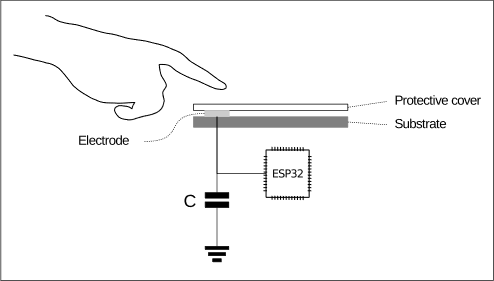
\includegraphics[scale=0.8]{images/FW/esp_touchsensor.PNG}
    \caption{ESP32 built-in touch sensor}
    \label{fig:esp_touchsens}
\end{figure}

\newpage
    \subsubsection{Prototyping design}
For our prototypes, we have experimented with different test codes, different materials and different touch pad designs.

\paragraph{Touch pad design} For initial prototyping, we used simple cables connected to the microcontroller's pins. The tips of the cables could be touched triggering the touch sensors. We then used conductive fabric and conductive paint for prototyping touch pad design and interactions. The materials used for prototyping are described below.

\medskip
In the prototype for MS4, we had large conductive sensors made out of woven conductive textile \cite{conductivefabric}, as seen in figure \ref{fig:proto1}. In the second prototype, in order to reduce the area and increase the capacity of the touch sensors, we used cut-out heat-bond conductive pads \cite{heatbond} as illustrated in figure \ref{fig:proto2_sensors}.

\paragraph{Conductive materials} We experimented with conductive thread \cite{conductivethread}, knit and woven textile from Adafruit \cite{conductivefabric}, conductive paint from Bare Conductive \cite{bareconductive} and heat-bond conductive fabric from Less EMF \cite{heatbond}. The latter is the best in terms of manufacturability as it can easily be fixed to the soft PCB fabric and is not susceptible to fraying and creating short circuits. The conductive paint is great for prototyping and fixing small connectivity issues but is water-soluble so it will not be considered as a reliable manufacturing option for the prototype (if sealed in acrylic it may be considered, especially for manufacturing speed such as in silk-screen printing). 

    \subsubsection{Experimenting with soft sensors} 
We experimented several types of soft sensors and materials: bend sensors with Velostat \cite{velostat}; stretch and pressure sensors with Eontex \cite{eontex} and a potentiometer thread from Adafruit. After considering manufacturability, ease of integration, repeatability, interaction possibilities and costs, we decided to keep only the touch/press sensors.

\paragraph{Velostat bend sensor} The bend sensor, pictured in \ref{fig:softsens_bend}, was inspired byAdafruit's handcrafting guide for textile sensors \cite{textile_sensors}, page 7. The design is basically a piece of velostat resistive sheet "sandwiched" in between two layers of fabric with one layer connected to the ground, the other connected in parallel with a 50ohm resistor to an ADC input pin. As the resistivity of the velostat layer reduces when bent, the built-on analog-to-digital converter was able to pick up bending of the sensor translating as change in resistance. 
\newline However promising in results, this soft sensor was put aside as our designers couldn't find an appealing was to use them in the plush toy. Results from the test scenario can be found in appendix \ref{fig:velostat_graph}.

\paragraph{Eontex stretch sensor} In a similar way to Velostat, Eontex's resistance goes down linearly as the fabric is stretched. For this sensor, pictured in \ref{fig:softsens_stretch}, we connected one extremity to the ground and one to the ADC pin in parallel with a 50 ohm resistor. This sensor exhibited great properties when stretched, but had low repeatability, limiting the possible applications of this kind of sensors.  Results from the test scenario can be found in appendix \ref{fig:eontex_graph}.


\begin{figure}[H]
    \centering
    \subfloat[Velostat bend sensor\label{fig:softsens_bend}]{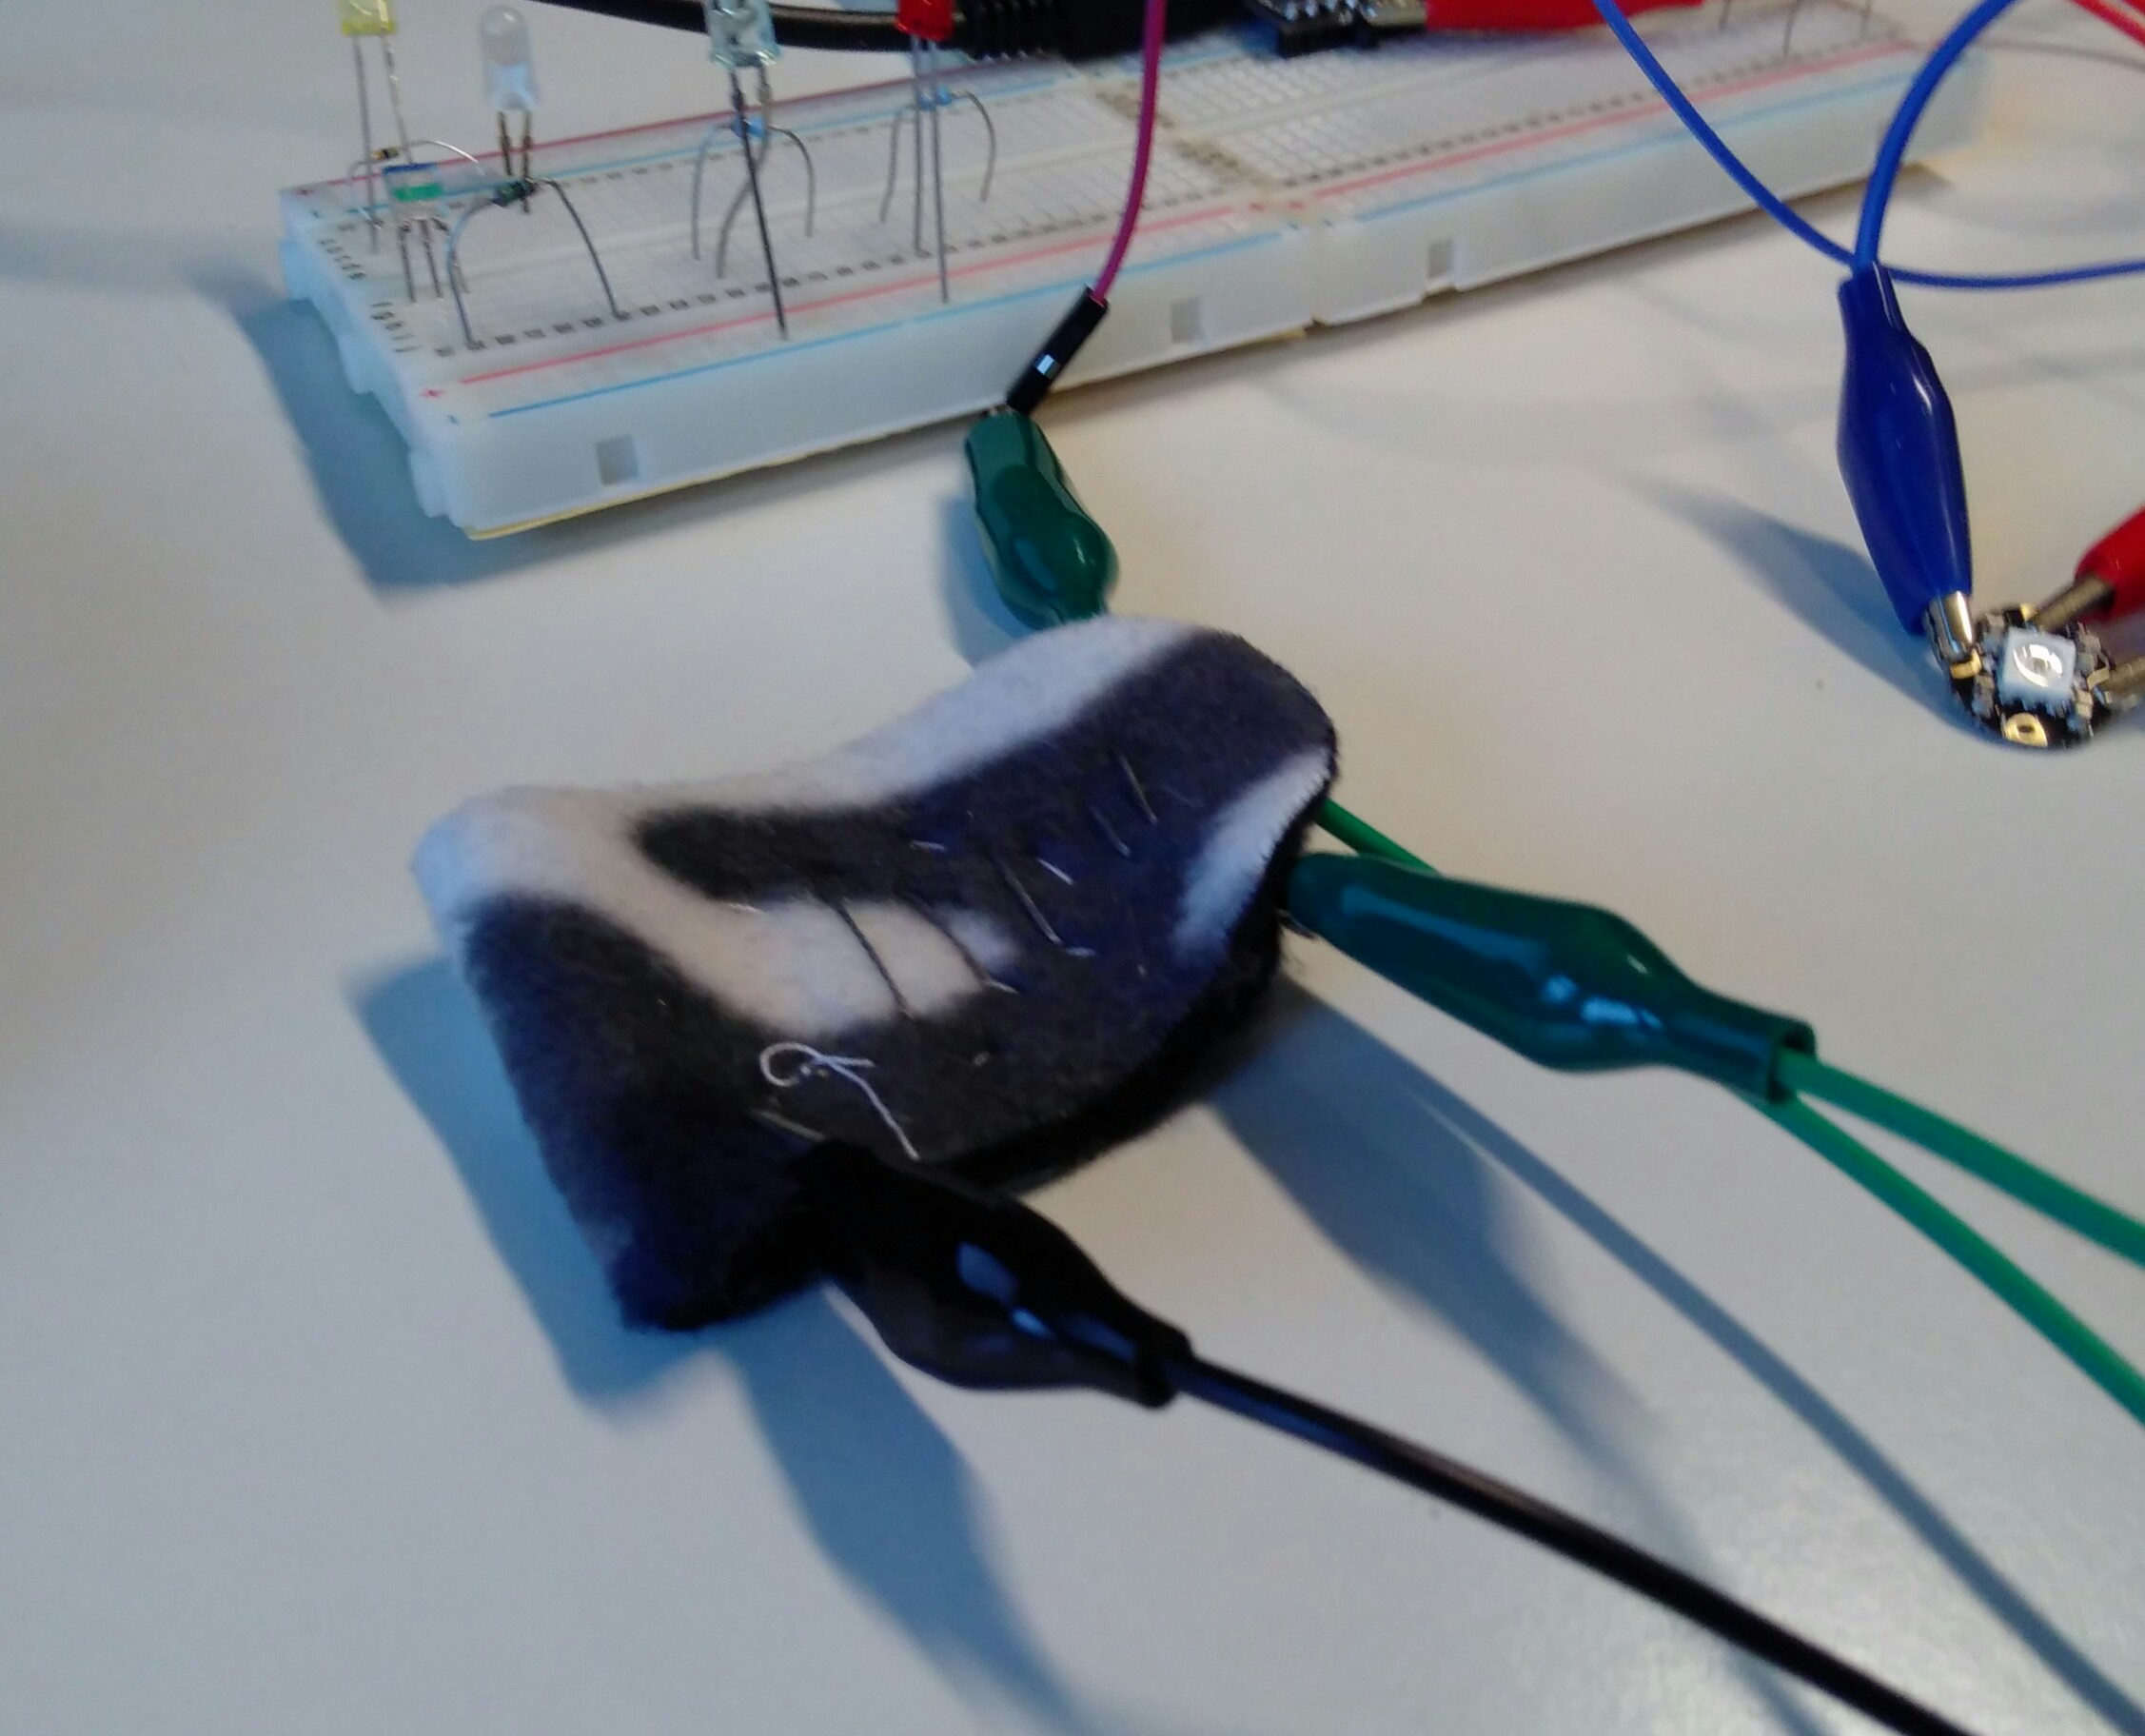
\includegraphics[width=0.47\textwidth]{images/HW/softsens_bend.jpg}}\hfill
    \subfloat[Eontex stretch sensor\label{fig:softsens_stretch}] {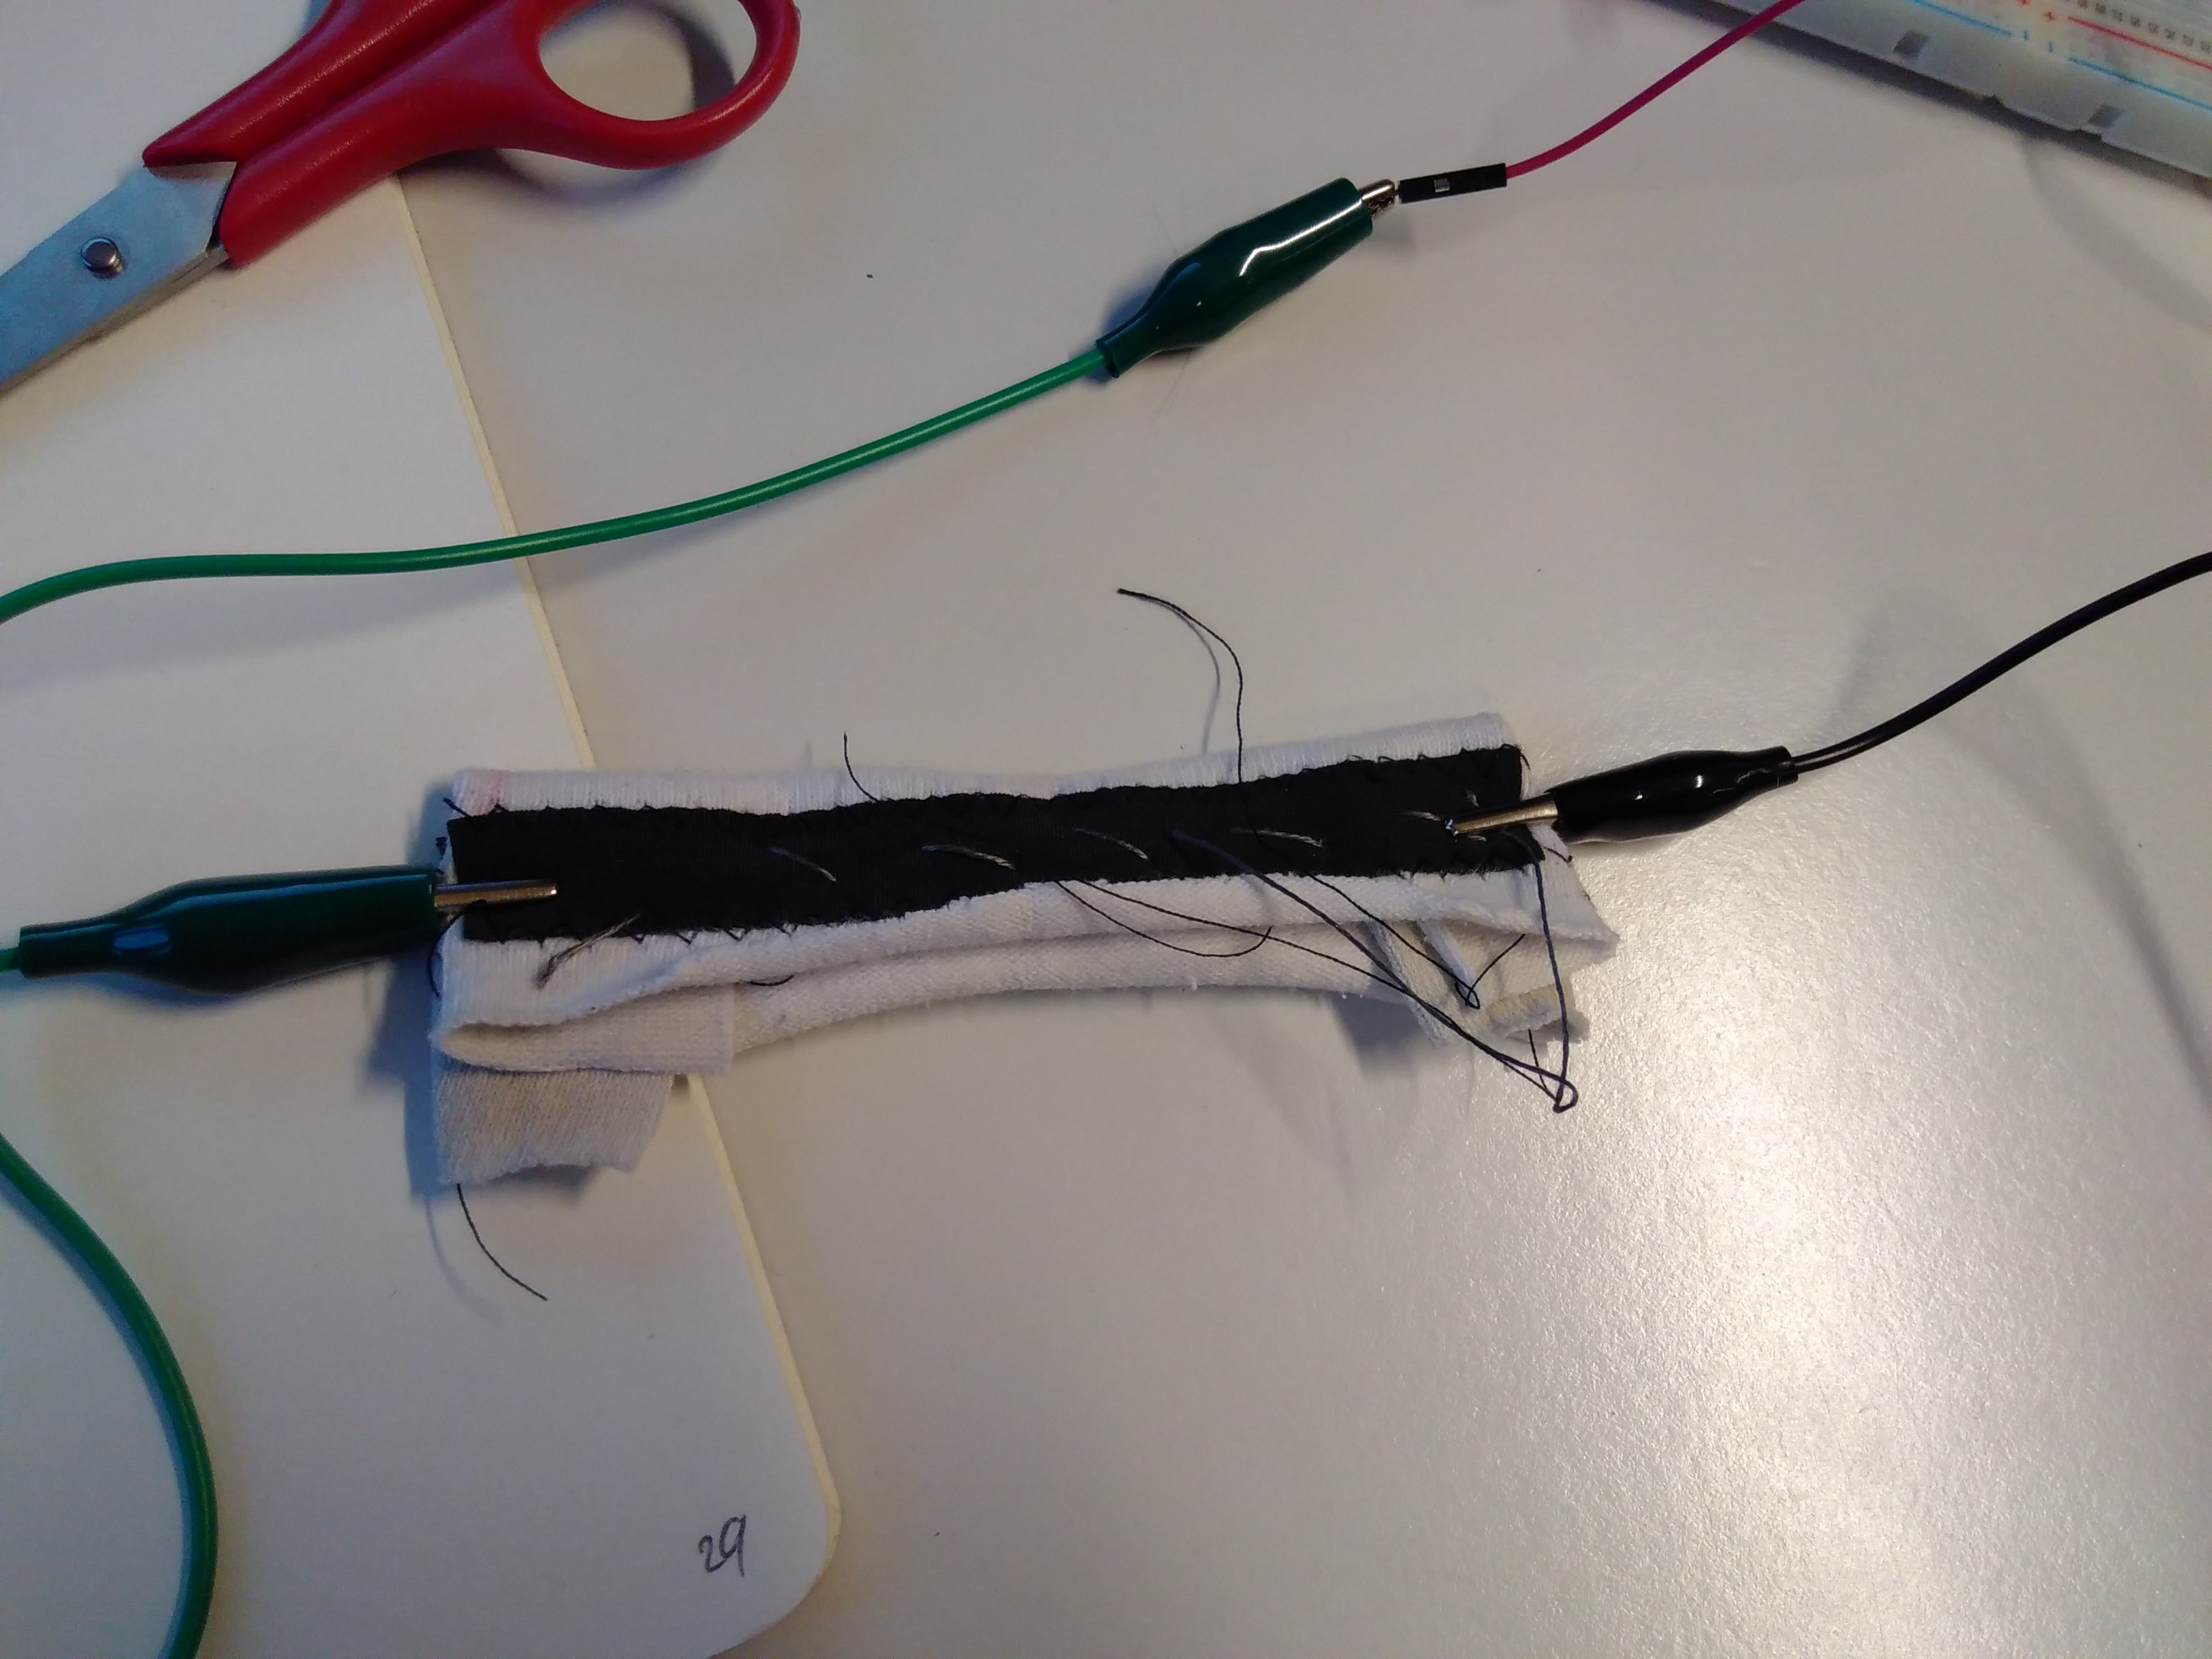
\includegraphics[width=0.47\textwidth]{images/HW/softsens_stretch.jpg}}\hfill
    \caption{Examples of two other soft sensors we experimented with} 
    \label{fig:softsens}
\end{figure}

\subsection{Hard <-> Soft interfaces}
In our first prototype, we used banana cables attached to safety pins to ensure connectivity of the textile pads to the microcontroller. The second prototype had crimp pins attached to the conductive threads, illustrated in Figure \ref{fig:proto2_connectors}. The third prototype (MS6) will probably have the conductive threads/textile tracks attached to the secondary PCB.

\subsection{Next steps} For China or the next semester, we would like to have a compact, robust and user-friendly connector. Such connector could be designed with pogo pins on one side (PCB or textile) and connecting pads on the opposite side to ensure proper connectivity in a user-friendly and compact packaging. This design has been inspired by the connectors for different modules found in the Fairphone (Fig. \ref{fig:fp}).

\begin{figure}[H]
    \centering
    \subfloat[Pogo pin connector\label{fig:fp_connector}]{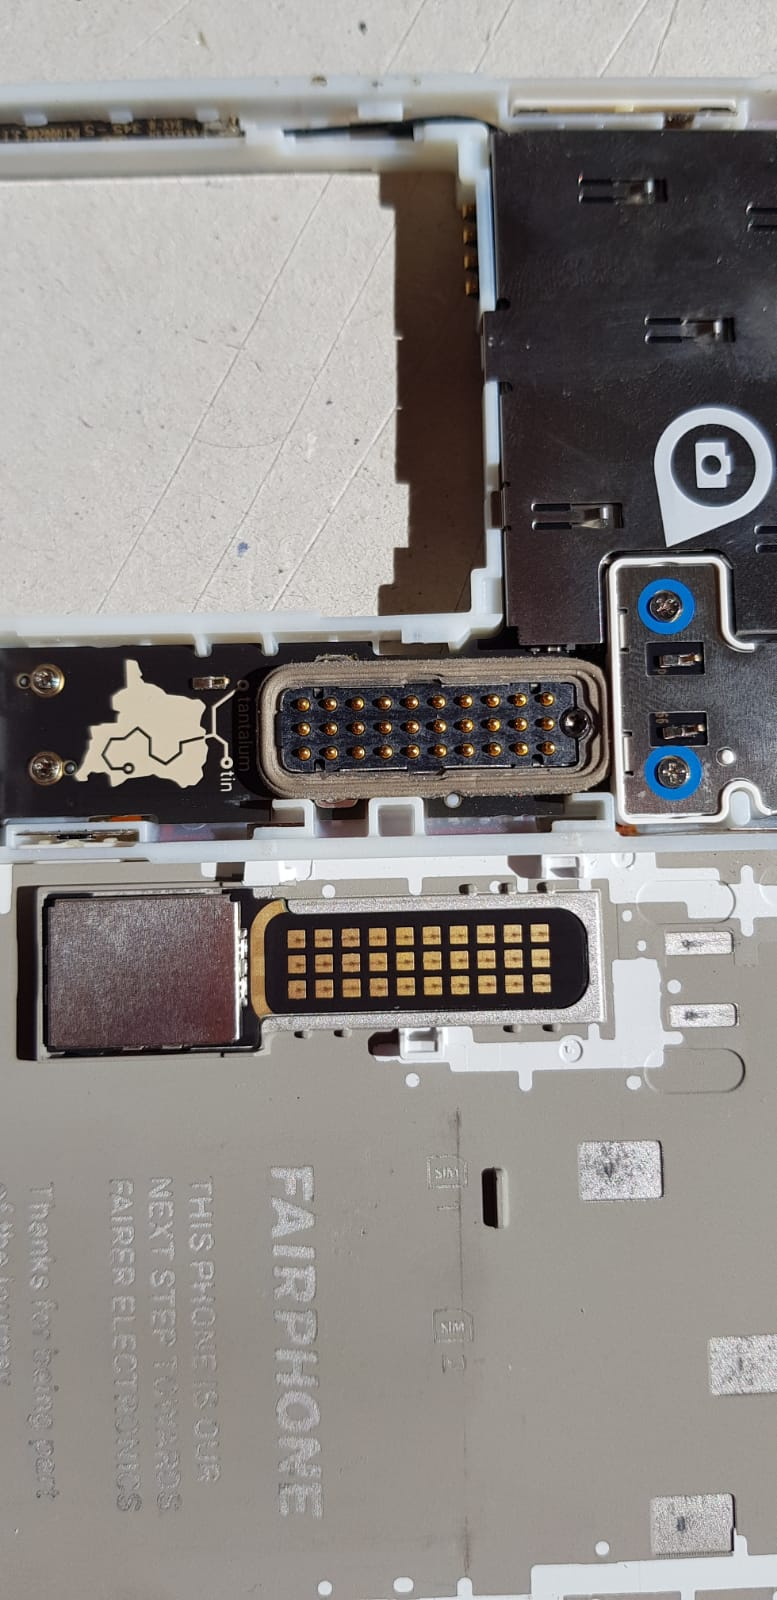
\includegraphics[width=0.4\textwidth, angle=90]{images/HW/FP_connector.jpg}}\hfill
    \subfloat[Connector with LED element\label{fig:fp_LED}] {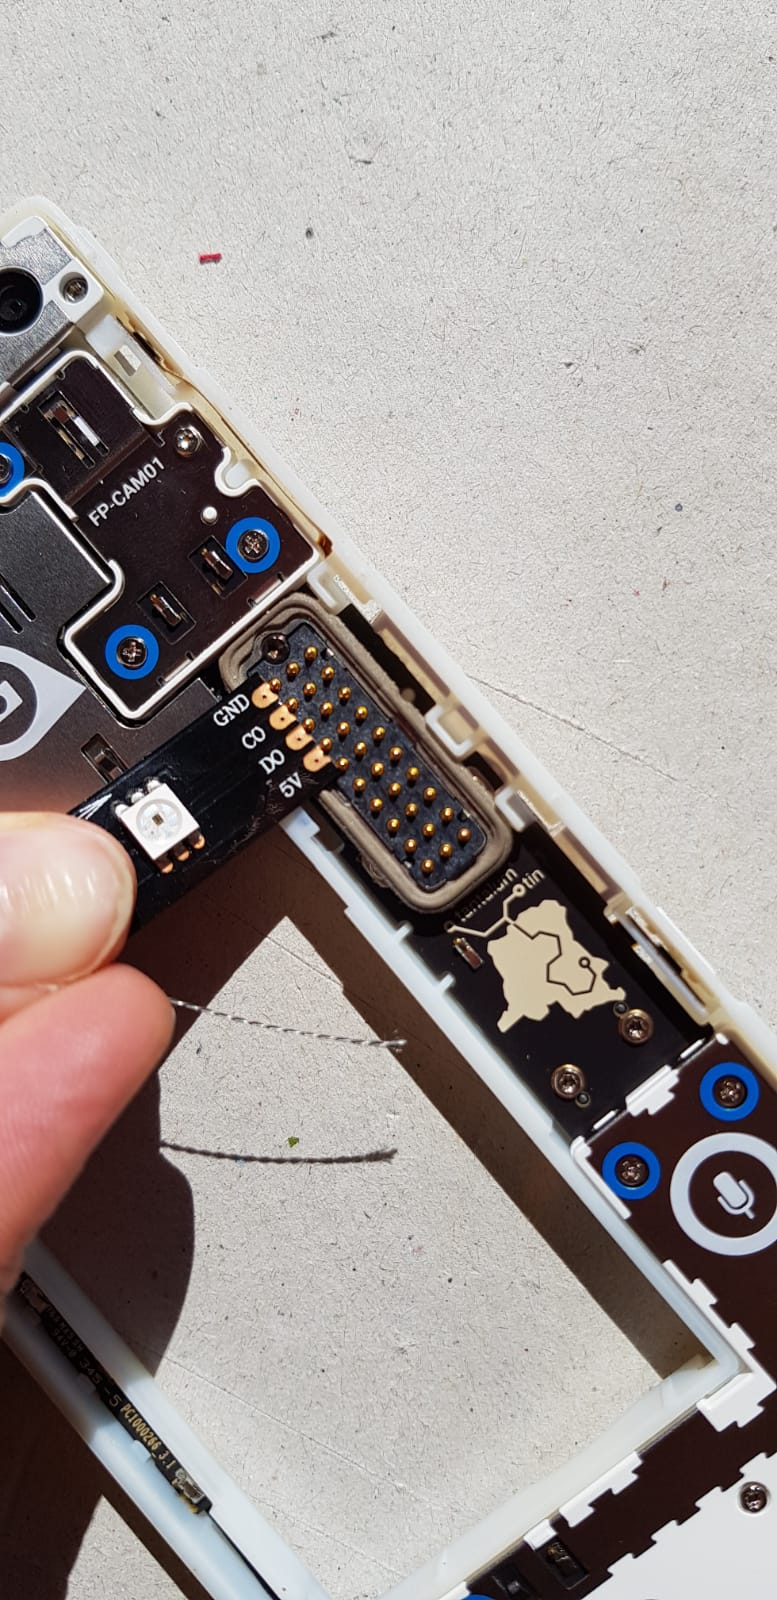
\includegraphics[width=0.4\textwidth, angle=-90]{images/HW/FP_connect_LED.jpg}}\hfill
    \caption{Example of pogo pin connector from the Fairphone's electronics} 
    \label{fig:fp}
\end{figure}